\documentclass[a4paper,12pt,twoside]{book}
\usepackage[utf8]{inputenc}
\usepackage[english]{babel}
%\usepackage{fontspec}
%\setmainfont[
%  Ligatures=TeX,
%  Extension=.otf,
%  BoldFont=cmunbx,
%  ItalicFont=cmunti,
%  BoldItalicFont=cmunbi,
%  SlantedFont=cmunsl
%]{cmunrm}

%\usepackage{polyglossia}
%\setmainlanguage{spanish}

\usepackage[c5paper]{geometry}
%\geometry{inner=2.5cm,outer=2.5cm,bmargin=3.2cm}
%\usepackage[DIV=14,BCOR=2mm,headinclude=true,footinclude=false]{typearea}

%\usepackage{ulem} %Hace que \emph sea subrayar

%\usepackage[p,osf]{scholax}
%% T1 and textcomp are loaded by package. Change that here, if you want
%% load sans and typewriter packages here, if needed

\usepackage{ebgaramond}
%\usepackage[type1]{libertine} % Linux Libertine for zweispaltige Texte
%\usepackage{textcomp}% Required to get special symbols
\usepackage[scaled=.8]{DejaVuSansMono}% FiraMono Typewriter font
\usepackage{PTSansNarrow} 
%\gilliuscondensed
%\usepackage[sfdefault]{FiraSans}
%\usepackage{bm}% Extra bold faces
%\usepackage[lf]{carlito}

\usepackage{lettrine} %Capital letters at the beginning of a chapter
\usepackage[activate={true,nocompatibility},final,tracking=true,kerning=true,spacing=true,factor=1100,stretch=10,shrink=10]{microtype}
\SetTracking{encoding={*}, shape=sc}{-20} % versalitas menos separadas
% activate={true,nocompatibility} - activate protrusion and expansion
% final - enable microtype; use "draft" to disable
% tracking=true, kerning=true, spacing=true - activate these techniques
% factor=1100 - add 10% to the protrusion amount (default is 1000)
% stretch=10, shrink=10 - reduce stretchability/shrinkability (default is 20/20)

%\usepackage{array,multirow,booktabs,colortbl,chngcntr} % El último es para counterwithout;
\usepackage[strict]{changepage}
%\usepackage{caption}
%\captionsetup{format=plain,labelsep=newline,labelfont={small,sc},
%textfont={small,it},singlelinecheck=false}
\usepackage[Bjornstrup]{fncychap} % Para cabeceras de capítulos sofisticados:     Sonny,    Lenny,    Glenn,    Conny,    Rejne,    and Bjarne.

\usepackage{graphicx,wrapfig,booktabs,multicol} % wallpaper: poner imágenes de fondo; wrapfigure: figuras a un lado del texto
%\graphicspath{{figures/}}
\usepackage{fancyhdr}
\usepackage{emptypage,pdfpages,fancybox} % Para que las páginas en blanco no tengan encabezado;
\usepackage{enumitem} %paralist: para compactenum, enumerate sin espacios
%\setlist[itemize]{nosep} %Espacio entre items en itemize
\usepackage[hyperref]{xcolor}
\usepackage[hidelinks]{hyperref}
\usepackage{xurl}

%\usepackage{minipage}

%\usepackage{quotchap} %Encabezados de capítulos
\usepackage{syntonly,verbatim}
%\syntaxonly

\usepackage{setspace,xspace} % xspace: Da \xspace para no tener que poner {} después de los comandos; pdflscape: páginas en horizontal;

\newenvironment{quotex}{\begin{quote}\small}{\end{quote}}
\newenvironment{quotationx}{\begin{quotation}\small}{\end{quotation}}


\begin{document}

% Por alguna razón, los marginados se creaban al revés. Así los corrijo. Feo, pero eficaz:
\let\tmp\oddsidemargin
\let\oddsidemargin\evensidemargin
\let\evensidemargin\tmp
\reversemarginpar

%\setcounter{secnumdepth}{4} % Para que llegue a numerar hasta las subsubsecciones;
%\renewcommand{\heavyrulewidth}{0.14em} % Grosor de las líneas extremas de las tablas;
%\renewcommand\thempfootnote{\alpha{mpfootnote}} % Símbolo de notas dentro de minipage
%\let\oldcaptionof\captionof
%\renewcommand{\captionof}[2]{\oldcaptionof{#1}{\newline \textit{#2} }}
%\renewcommand{\tablename}{Tabla}
%\counterwithout{figure}{chapter}
%\counterwithout{table}{chapter} % Así la numeración es 1, 2, 3... y no 1.1, 1.2... y no reinicia la num. en cada capítulo;

%\providecommand{\ggl}{\guillemotleft}
%\providecommand{\ggr}{\guillemotright\xspace}
\providecommand{\flright}[1]{\begin{flushright}#1\end{flushright}}
\providecommand{\flrightit}[1]{\begin{flushright}\itshape #1\end{flushright}}
%\renewcommand\UrlFont\sffamily
\urlstyle{tt}

\pagestyle{fancy}
\renewcommand{\sectionmark}[1]{\markright{#1}}
\renewcommand{\chaptermark}[1]{\markboth{#1}{}}

%Portada:
%\includepdf{00Portada}

\frontmatter
%
%\onehalfspacing
%\pagenumbering{Roman} %gobble es como empty

%\include{preindice}

%\fancyhf{}
%\fancyhead[LE]{\small \textbf{\thepage}$\quad$ Índice general}
%\fancyhead[RO]{\small Índice general $\quad$\textbf{\thepage}}
%\clearpage
\tableofcontents

%\doublespacing
\mainmatter

\fancyhf{}
\fancyhead[LE]{\small \thepage$\quad${\scshape\chaptername{} \thechapter}: \nouppercase{\itshape\leftmark}}
\fancyhead[RO]{\small \textsc{Section }\thesection{}: \nouppercase{\itshape\rightmark} $\quad$\upshape\thepage}
%\cfoot{\bfseries\thepage}

\pagenumbering{arabic}

%\onehalfspacing

% introductorios

\chapter{Introduction}
\section{The Owl of Minerva}

\begin{quotex}
The owl of Minerva flies at dusk.

\end{quotex}
\paragraph{Seeing in the Dark}

\begin{wrapfigure}{tr}{.25\textwidth}
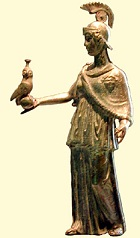
\includegraphics[scale=.9]{a20110630TheOwlofMinerva-img001.jpg} 
\end{wrapfigure}

This proverb from Hegel means that philosophy can only understand a cycle at its end. Hence, it is not helpful at its beginning, so anyone who is now engaged in the “battle of ideas” can hope for little more than a pyrrhic victory at best. Rather, it is a struggle of visions or world views. Pace Hegel, the Owl of Minerva is not a philosopher. The owl is wise not because he can think but rather because he can see in the darkness. While the world sleeps, the owl is vigilant at night. Thus, the men of Tradition must also be vigilant during the darkness.


At the beginning of a cycle, there is no need for philosophy. Man lives in immediacy following his Tradition faithfully and there is no need for questioning, and no need for wonder which is the motivation for philosophy. Unperturbed by the conflicts of competing thoughts, he lived with certainty. When an issue arose, he didn't think about it. Rather he followed the Tradition of his ancestors and his gods without question. His moral code was duty to the city, family, and gods. This code prescribed all his actions, which had to be executed precisely, and there was no room for subtleties. These rites maintained the souls of his ancestors and brought their blessings; he expected his sons to do the same for him after his death. These civilizations lived in relative internal harmony, sometimes for millennia.

Only with the decline of a cycle does thought arise. The corrosive effect of discursive thought calls everything into question. It no longer suffices to follow the ancestors and gods, one must also give a reason for doing so. Those skilled at logical and creative thinking become the philosophers. They offer their services to men in search of understanding. Others, such as the Sophists, notice that thought is an end in itself and can be used for persuasion apart from its actual truth value. The Sophists are the first propagandists and sell their services.

\paragraph{Three Civilizations}
\begin{quotex}
…bisogna tener ben fermo questo punto, indispensabile per una formulazione imperiale e romana dell'idea razzista e confermato da ciò che fu proprio alle grandi civiltà arie d'Oriente, all'antica Roma, al Medioevo romano-germanico.

\end{quotex}
We are focusing on the civilizations of the Borean race, as Fabre d'Olivet called it, who origins were in the mythical Hyperborea, whence it spread to India, Central Asia and Europe. There is not the time or energy to deal with the traditions of Asia, Africa, or the Amerindians. Furthermore, we have been focusing on just three Borean civilizations of a traditional nature, omitting the Nordic and Celtic traditions which are no less important. But since Julius Evola identified them as the three main civilizations of Indo-Eurpean origin, they serve as a good basis for discussion.

\begin{description}
\item[Hyperborea ]

We can get a glimpse into these people only through extrapolation. By the interpretation of myths we can try to reconstruct their society. For this, we are relying on \textbf{Bal Tilak}, \textbf{Fabre d'Olivet} and \textbf{Herman Wirth}. 

\item[Bharat Khant ]

Bharat Khant was the ancient name for the Vedic civilization of India. This is the oldest group that we have documentation for, which includes the Vedas and the Laws of Manu. It is most important for us today because of its rich metaphysical tradition which comprise the six orthodox schools, all deriving from the Vedas. This should not uncritically be confounded with the contemporary religion of Hinduism. Unlike Hinduism, the Vedic civilization included ancestor worship, animal sacrifice and rejection of reincarnation. 

\item[The Ancient City ]

By this, we mean the ancient city-states of Greece and Italy. Although their origins are obscure, their traditions and eventual decline are reasonably well documented. That makes their study invaluable to those of use seeking the light hidden by the darkness. 

\item[Christendom ]

Instead of circumlocutions such as “Medieval period” and the like, we will use this term to describe the civilization that arose in Europe following the fall of Rome, without intending by that term to impose a particular theological interpretation on it. To put a time frame on it, we mean the approximate thousand year reign from Constantine to the Reformation, which united spiritually much of Europe. We will see that it had its declines that mimicked the decline of the Ancient City, at least in principle if not in detail. But here we have the added advantage that its origins are also documented. Thus, we can see what it adapted from its predecessor and what it rejected. This will serve as a useful model for a new cycle. 

\end{description}
\paragraph{Three Types of Men}
Each period was marked by a special type of man who embodied its superior aspects. These were never theoretical men, or those with the “best idea”, but men of a higher knowledge, a direct knowing or gnosis that can never be fully encompassed in thought. The knowing took various forms.

\begin{description}
\item[The Seer ]

The type of the Vedic period was the \textbf{Rishi} and the \textbf{Yogi}. The Rishi, or seer, had clairvoyant vision to see into the nature or essence of things beyond the accidental, incidental, or the trivial. The Yogi was the man of power: for bhakti yoga, power over the emotions; for karma yoga, power over one's actions; for jnana yoga, power over one's mind. The jnani, or knower, was master of his mind. By transcending the stream of thoughts, which held no more significance to him than the movement of clouds across the sky, the jnani gained direct insight into the nature of things. 

\item[The Hero ]

The Hero of the Ancient City was the \textbf{Hero}, the patriarch of a family, the founder of the city. As priest, he was the link between the gods and men and had the power to invoke their blessings. As king, he had the power of command over men. He had the power to interpret the omens, because in order to predict the future, he had to create the future. 

\item[The Believer ]

Christendom began where the Ancient City left off, in particular, it separated the roles of priest and king, without, however, secularizing the latter as had been done in the successive revolutions of the previous era. This leads to two different figures, united in faith, although different in temperament. These are the Saint and the Knight. Rather than seeking godhood by means of the rituals and sacrifices of their sons as in the age of heroes, they relied on their respective devotions to the True God and the True Man. The \textbf{Saint} through his ascetical practices was drawn toward theosis (divinization). The \textbf{Knight} of heroic valor followed the path of the Fedeli d'Amore to lead to the alchemical marriage. 

\end{description}
\paragraph{The Way Forward}
\begin{quotex}
Io ho difeso e difendo idee … nella misura in cui riprendono una tradizione superiore e anteriore … in quanto appartengono al retaggio della carattere universale e mantenutasi in Europa fino all Rivoluzione francese. Nello stesso spirito … dei grandi filosofi cattolici del principio di autorità, de Maistre e Donoso Cortes … I miei principi sono solo quelli che prima della Rivoluzione francese ogni persona ben nata considerava sani e normali.

\end{quotex}
The way forward is indicated by Evola as quoted above: to defend the higher traditions of Europe that every well born person considered sane and normal. We need not look back to the distant past, just to Europe before 1789 since these principles have a universal character. To reject these principles, as those of the new right seem to do, is to squander our legacy and dishonor our ancestors. If anyone is unclear about those principles, please read Donoso Cortes’ essays\footnote{\url{https://www.gornahoor.net/library/CortesEssays.pdf}}, as Evola recommends.

The way forward is based on authority as illustrated by our examples. In future posts we will lay out some programs described by \textbf{Fabre d'Olivet} and \textbf{Saint-Yves d'Alveydre} based on theocracy, Synarchy and the spiritual unity of Europe. But ultimately, it will depend on men of vision, seers, heroes, and those of unshakable faith.

\flrightit{Posted on 2011-06-30 by Cologero}

\chapter{Hyperborea}
\section{Hyperborea and the Primordial Tradition}

\begin{quotex}
In general, the men whom pride makes melancholy, always discontented with the present, always uncertain of the future, love to reflect upon the past from which they believe they have nothing to fear; they adorn it with smiling colours which their imagination dares not give to the future. They prefer, in their somber melancholy, superfluous regrets without fatigue to real desires which would cost them some efforts. \flright{\textsc{Fabre d'Olivet}}

\end{quotex}
\paragraph{Introduction}
There exists an egalitarianism of thought, whose presumption is that human consciousnesses are fundamentally alike, both across time and also across the different strata within society. But this is irreconcilable with some fundamental metaphysical principles\footnote{\url{https://www.gornahoor.net/?p=823}}: the doctrine of cosmic cycles presumes a difference over time (diachronic) and the doctrine of castes presumes a difference within time (synchronic).

Previous writers on Tradition have not always drawn out fully the consequences of these doctrines. Their view has been static and treated the various traditions as though they were mushrooms arising spontaneously after the rain. The consequence has been that ``tradition" often devolves to a type of comparative religion with debates about which tradition is the ``best" or more ``suitable", and so on, based on little more than contingent historical events or polemical ``sound bites". Instead, these doctrines should throw light on why certain forms appeared where and when they did and what is the relationship to each other. The Western or Roman Tradition is the evolution of the Hyperborean Primordial Tradition\footnote{\url{https://www.gornahoor.net/library/UltimaThule.pdf}} (understood as the unfolding in time due to the forces of cosmic cycles). Thus, we trace the development from the North to the East to the South and to the West. Then, towards the end of a complete cycle, the full effects of the Kali Yuga being to manifest. There are reasons for all this.

\paragraph{Diremption and Man}
The appearance of man brought about a diremption in the cosmos. This split Heaven from Earth, with Man as the reconciling force. Initially, the consciousness of man had direct intuitive knowledge of both Heaven and Earth; the soul, or psyche, was experienced as a life force or elan vital, rather than the complex of thoughts, feelings, likes, dislikes, images and so on, that trap man in subjective isolation.

\paragraph{Primordial State}
In contrast, the Hyperboreans in the Primordial State would have lived in purity (undivided mind and will) in the light of the sun followed with long nights interspersed with a dim light on the horizons where the sun is struggling to rise or set.

There is abundance to satisfy all needs, the Hyperborean knows when he is satiated. The mind is free of fear, worry, anxiety. Death is experienced, not as destruction, but rather as a transformation to a different state.

There is an intuitive awareness of God and the universal order by clairvoyant vision, just as we now recognize a tree or a mountain by direct experience. Thinking is regarded as another sense, along with sight, hearing, touch or taste. Discursive thought — of the ``yes" and the ``no", of the ``good" and the ``evil" — is not present. Instead, thoughts are experienced as voices from the celestial hierarchies (gods or angels) or communications from ancestors or as commands from rulers.

Knowledge is passed on by myths, symbols, and rites, in poetic forms.

Temporal power is exercised without force and obeyed willingly; the structure of society is held together by bonds of loyalty, family, and love. Commands are experienced, not as an imposition from the outside, but rather as the direct revelation of spiritual authority in one's own consciousness.


\hfill

Recommended reading

\begin{itemize}
\item Anonymous, \emph{Meditations on the Tarot} 
\item Antoine Fabre d'Olivet \emph{Hermeneutic Interpretation of the Origin of the Social State of Man} 
\item Arthur Branwen, \emph{Ultima Thule: Julius Evola e Herman Wirth} 
\item B G Tilak, \emph{The Arctic Home in the Vedas} 
\item Julian Jaynes, \emph{The Origin of Consciousness in the Breakdown of the Bicameral Mind} 
\item Rene Guenon, \emph{The Great Triad} 
\item Rudolf Steiner, \emph{Spiritual Beings in the Heavenly Bodies \& in the Kingdoms of Nature} 
\end{itemize}


\flrightit{Posted on 2011-01-09 by Cologero }

\begin{center}* * *\end{center}

\begin{footnotesize}\begin{sffamily}



\texttt{James O'Meara on 2011-01-09 at 21:36 said: }

``Previous writers on Tradition have not always drawn out fully the consequences of these doctrines. Their view has been static and treated the various traditions as though they were mushrooms arising spontaneously after the rain. … Instead, these doctrines should throw light on why certain forms appeared where and when they did and what is the relationship to each other."

Oddly enough, I was re-reading Revolt Against the Modern World this weekend, and it occurred to me that this is exactly what makes Evola distinctive. Part One constructs a model of ``Tradition" derived from a survey of world traditions, using a method of synthesis [``the Traditional Method"] which I've previously compared to such methods as [here] to Spengler's ``physiognomic tact" and [on my blog] Clive Bell's artistic sense. Part Two then surveys actual [well, according to him] historical developments, identifying various `cycles.' as Tradition interact, declines, recoups, etc. 

By contrast, Schuon is the anti-Evola, taking each tradition as a `mushroom' or a-synchronic whole [``The Christian", ``The Taoist" etc.]. H. Smith took this model and calcified it further, if possible, into a cookie-cutter eso/exo model for all world religions, taken as such with no analysis at all.

This is exactly what made Evola so interesting, both theoretically as well as in practice [his attempts to influence contemporary events], after coming from reading Guenon etc., who by contrast seem like armchair theorists. 

Schuon take everything today as given, and accounts for change or conflict by the all-purpose `divine adaption.' Evola, and even Guenon, are able to dig beneath the surface and explain, say, the Roman tradition as an ongoing reconquest of telluric influences by a Nordic cycle etc.


\hfill

\texttt{Mark on 2011-01-10 at 16:00 said: }

I will post here to comment on Kadambari's comment that Putin has declared Russia an Orthodox country. The reality is that the adoption of Christianity by the Northern peoples has caused a rupture in their spirit. Their pagan imagination has a tendency to want to go to deeper myths.

\url{http://onlinelibrary.wiley.com/doi/10.1111/j.1469-8129.2008.00329.x/abstract}

``ABSTRACT. As in all post-Soviet states, the Russian intelligentsia has been preoccupied with the construction of a new national identity since the beginning of the 1990s. Although the place of Orthodox religion in Russia is well documented, the subject of neo-paganism and its consequent assertion of an Aryan identity for Russians remains little known. Yet specialists observing the political and intellectual life of contemporary Russia have begun to notice that the development of references to `Slavic paganism' and to Russia's `Aryan' origin can be found in the public speeches of some politicians and intellectual figures. This article will attempt, in its first section, to depict the historical depth of these movements by examining the existence of neo-pagan and/or Aryan referents in Soviet culture, and focusing on how these discourses developed in different spheres of post-Soviet Russian society, such as those of religion, historiography, and politics."

\url{http://www.springerlink.com/content/j30056125185344h/}

Perun's revenge: Understanding theduxovnaja kul'tura

The one thing that it seems that Kadambari has not been able to appreciate is the fact that a Christian conscious and a ``Pagan" unconscious has affected the people of the North in a different way than the people of the South.

It has interested me as to why the synthesis of Paganism and Christianity has caused a rupturing in the person of the North to the point where if we take someone from Scandinavian descent, if they take their religion seriously, then they become either a fundamentalist Protestant or Asatru, whereas this does not arise as much in the Greek or Italian.


\hfill

\texttt{Cologero on 2011-01-10 at 18:47 said: }

That is an interesting point, Mark. I have a post in mind that explores that very topic, though I've delayed it because it is inconclusive. Perhaps, I'll post it anyway, after a little preparation.


\hfill


\end{sffamily}\end{footnotesize}

\section{Arctic Home in the Vedas}

\begin{quotex}
From the dead sun springs a daughter more beautiful than her sire, and mankind starts afresh from the life-raiser and his bride-Life. 

\end{quotex}

In which we briefly outline the idea of cosmic cycles, and illustrate them initially in the revelation of the originary Hyperborean source of the Vedas. This is then extended to Traditions following the Vedas. Finally, there is some speculation on the future course of the West. The foundation is the book \textit{The Arctic Home in the Vedas} by \textbf{Bal Tilak}.

\paragraph{Cosmic Cycles}
Since a more complete exposition can be found in Rene Guenon's writings, from whom these notes are taken, and elsewhere, we provide here just the most basic outline.

\textbf{Cycle}: represents the process of development of some state of manifestation

\textbf{Minor cycle}: one of the more or less restricted and specialized modalities of that state

Since the \textbf{Law of Correspondence} links all things in universal Existence, is necessarily and always a certain analogy, either among different cycles of the same order or among the principal cycles and their secondary divisions

\textbf{Kalpa}: total development of a world. One cannot speak literally about its duration so that duration has a purely symbolic value. Perhaps not in our world because time is one of its determining conditions.

\textbf{Manu}: there are 14 Manus, each ruling over a Manvantara. There are two septenary series. The first septenary is that of descent, or devolution, and includes ours. The second is ascent or evolution.

\textbf{Manvantaras}: cycles have a character that is both cosmic and historical, they concern terrestrial humanity, also linked to events occurring outside the history of humanity. There is a correlation between the cosmic and human orders. This means, for example, that events in the human realm correspond to events in the celestial spheres.

These relate to the 7 \textbf{svargas} and 7 \textbf{patalas} which represent states respectively higher and lower than the human state. By correspondence, these can be related to the 14 manus.

\begin{wrapfigure}{rt}{.3\textwidth}
 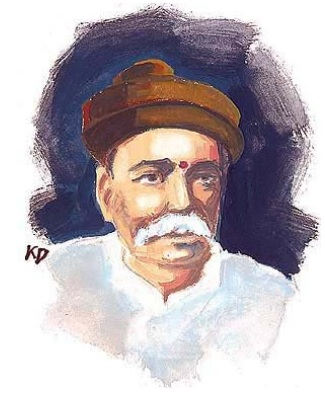
\includegraphics[scale=.5]{a20200723ArcticHomeintheVedas-img001.jpg} 
 \caption{Bal Tilak}
\end{wrapfigure} 

A Mantavara is subdivided into 4 \textbf{yugas}. We are allegedly in the last yuga, the Kali Yuga. The starting date and exact duration are not known, according to Rene Guenon.

There are 7 \textbf{Dvipas} or regions into which our world is divided. They are represented as islands or continents, but not parts of present-day earth. They may also refer to planetary spheres.

These ages, states, and regions also have symbolic meanings, since there is a sacred geography as well as a profane geography. Henry Corbin discusses this topic in his books, and it is also confirmed by Rene Guenon:

\begin{quotex}
There is also a symbolical geography; indeed, in this connection, there is a very significant correspondence between the domination of the West and the end of a cycle, for the West is the place where the sun sets. 

\end{quotex}
Thus, when he mentions the distinction between Eastern and Western understanding, this is no way simply a geographic distinction; i.e., there is no ``magic dirt" in the East. Guenon amplifies the idea:

\begin{quotex}
To the extent that a man `Westernizes' himself, whatever may be his race or country, to that extent he ceases to be an Easterner spiritually and intellectually. 

\end{quotex}
The converse is also true. Unfortunately, this is too often overlooked so there are some who fantasize about going east to find an ``initiatic centre" or give up entirely. Often, they justify this decision because of the ``corruption" they see in the Church hierarchy, as though India and Egypt are free of such corruption. These masters of ignorance have a loud presence on social media. The truth is that real initiates like Savonarola, Boccaccio, and Dante were complaining about corruption in the Church a thousand years ago. (See Canto XXI, \emph{Paradiso}, for example.)

How, then, could Dante describe his spiritual journey? His passage through Purgatory and Heaven are descriptions through the higher and lower stages. Guenon provides us with the general idea, but we need to get the details from others who have made the trip.

\paragraph{Hyperborean Migration}
The idea of a migration of a branch of the Borean race from a polar region to India has been a mainstay in esoteric literature. That is now considered outré and dismissed as the ``Aryan Invasion Theory". Times change. Bal Tilak, the author of The Arctic Home in the Vedas, was a Hindu nationalist and considered himself to be Aryan; so, it is not a Nazi fantasy. Perhaps there is no genetic, archaeological, or documentary proof. Nevertheless, as Georges Dumezil documented, there is still the trifunctional social organisation from Scandinavia, across Europe, to India that needs to be explained. Moreover, there is similarity in the mythologies of the various Indo-European people.

In any case, it may be best to regard Hyperborea as transcendent geography or one of the seven Dvipas. That is how the Greeks understood it, since only the gods could visit it. Apollo would arrive there by a swan.

Nevertheless, Tilak probes through the Vedas looking for clues for an actual migration several millennia ago. In particular, he sees astronomical facts that match the experience of a those living in a land close to the North Pole. For example, the original Roman calendar had 10 months, ending in December. That is because it would be followed by two months of darkness during which days could not be counted. It continues in that vein, relying as much on Western scholars as on the Vedas themselves.

Sometimes it gets tedious, much like exegesis on Genesis; is a ``day" 24 hours or does it refer to an age? Nevertheless, it is worth the trouble because of the vast amount of information in it.

The Vedas are eternal and without beginning. However, we owe the textual version to the seven Rishis who could ``see" the vedas from the beginning of the Kalpa. A deluge had destroyed the Vedas at the end of the previous Kalpa. Tilak's method is to juxtapose the Theological view in the Vedas with a corresponding Historico-scientific view gathered from external and profane sources. He also relies on comparative mythology relating Celtic, Greek, Roman, and Egyptian myths to corroborate the Vedic myths. Most importantly, Tilak regards the Zend Avesta, the sacred text of the Zoroastrians, as authoritative.

\paragraph{The Divine Word}
Since, this is an introduction, we can only point out some highlights; maybe someday we can do a more exhaustive review. This is an important point:

\begin{quotex}
Vedic names and forms of species are eternal, and it is by remembering these that the world is created by Brahmâ at the beginning of each Kalpa. The Veda is, therefore, the original WORD, the source from which everything else in the world emanated, and as such it cannot but be eternal. 

\end{quotex}
Tilak points out that this doctrine is tantamount to the notion of the divine \emph{Logos} of the Alexandrian school.

The duration of the various ages or yugas were in dispute. For example, by an early reckoning, the Kali Yuga would have ended soon after the birth of Christ. Although they knew nothing of that event, the authors of the Puranas in the first centuries AD, refused to believe the Kali Yuga had ended. Hence they extended the duration from 1000 human years to divine years (360 human years). Tilak points to similar artifices to fudge the dates for various purposes. The alternative is to assume that the Christian Era represented the end of the Kali Yuga and the beginning of an ascent.

The point is that the authors preferred to understand the ages by their qualities, not merely as the passage of quantitative time. Also, the original timeframes were much shorter than the fantastical extended duration of the ages that get passed around today.

\paragraph{Excursus on Method}
Tilak is very thorough, although the text points out the difficulty of fully understanding the Vedas in all cases. Both Evola and Guenon accepted Tilak's thesis; the latter actually thought very highly of Tilak. Guenon reveals some contradictions in his doctrines that require explanation. For example,

\begin{itemize}
\item Guenon claims Tilak was a non-Westernized Hindu. \textbf{FACT}: Tilak was quite familiar with European science, history, and mythology. Moreover, he had deep respect for the German Indologist, Max Müller. 
\item Guenon tediously rails against ``profane" science, history, philosophy, etc. \textbf{FACT}: Tilak relied heavily on those ``profane" fields of study to fortify his thesis. 
\item Guenon hates Vivekananda, but loves Tilak. \textbf{FACT}: Vivekananda was esteemed by not just Tilak, but even Hindus in India to this day. 
\end{itemize}
The point is that it is a mistake to disdain ``profane" scholarship when it might be helpful. By the Law of Correspondences, science and metaphysics should not be in conflict since they deal with different levels of existence. Guenon has done us a great service by his explanations of metaphysics and symbolism, by his deep comparisons of different traditions, and by expanding our understanding to include the full range of authentic human spirituality. There is no ``Guenonian doctrine" per se, since he is just rephrasing the doctrines of traditions that pre-existed him.

At the end of the day, Guenon does not judge Tradition; Tradition judges Guenon. That is lawful, not a negative judgment.

\paragraph{Traditional Forms}
It is one thing to mention the possibility of different stages/regions/states, etc., and quite another to fill in the details. That would perhaps require another Rishi, not for a new revelation, but rather for a deeper understanding. Tilak gives us some clues about how the different stages of Tradition might look.

The Letters to the Seven Churches in the Book of Revelation represent the seven stages of the development of Tradition. The following list represents Valentin Tomberg's understanding of the stages. This list is remarkably consistent with Tilak's exposition of the Vedas, with some speculation about the future.

\begin{enumerate}
\item \textbf{Ephesus}: The old Indian (Vedic) culture. This is primal revelation given to the Rishis in India. 
\item \textbf{Smyrna}: The old Persian (Zoroastrian) culture. The Zend Avesta also retained a memory of the Hyperborean revelation. 
\item \textbf{Pergamos}: The Chaldean-Egyptian (Hermetic) culture. This is based on the revelation of the Logos to the Alexandrian school. 
\item \textbf{Thyatira}: The Greco-Roman (pagan) culture. Although the Greeks retained some memory of Hyperborea, much came through Egypt. The Greeks had the same understanding of ``name and form" from Vedic metaphysics, despite the different emphases of Plato and Aristotle. 
\item \textbf{Sardis}: The Anglo-Germanic (Christian) culture. The Christian religion transformed Europe with a deeper revelation. Building on the Vedas and Hermetics, it understood the Logos as not just the creator, but also as equal to God as well as saviour and judge. Christianity got its philosophy from the Greeks and its Theology was enriched by the Alexandrian school as Vladimir Solovyov pointed out. 
\item \textbf{Philadelphia:} The Slavic-Russian (also Christian) culture. The Slavic nations should be the preservers of Tradition. We shall see how that plays out. 
\item \textbf{Laodicea:} The American, i.e. Western Hemisphere, (future) culture. North and South America will look quite different in the future. More cannot be said at this time. 
\end{enumerate}
There are three churches of the past, two of the present, and two of the future. But do not take the history and geography too literally, for they represent streams that are always active in us.



\flrightit{Posted on 2020-07-23 by Cologero }

\begin{center}* * *\end{center}

\begin{footnotesize}\begin{sffamily}



\texttt{Christopher on 2020-07-23 at 15:48 said: }

``Guenon tediously rails against ``profane" science, history, philosophy, etc. FACT: Tilak relied heavily on those ``profane" fields of study to fortify his thesis."

While I agree generally with the tediousness of Guénon in this regard, I don't believe it to be a contradiction. Guénon has, at various times, cited archaeological findings (his article on La triple enceinte druidique comes to mind) and defended the potential use of profane archaeology, even while criticizing its current usage. In his article on the Place de la tradition atlantéene dans le Manvantara (Le Voile d'Isis, August–September 1931), he wrote:

« On ne saurait être trop prudent quand il s'agit de civilisations entièrement disparues, et ce ne sont certes pas les tentatives de reconstitution auxquelles se livrent les archéologues profanes qui sont susceptibles d'.claircir la question ; mais il n'en est pas moins vrai que beaucoup de vestiges d'un passé oublié sortent de terre à notre époque, et ce ne peut être sans raison. Sans risquer la moindre prédiction sur ce qui pourra résulter de ces découvertes, dont ceux qui les font sont généralement incapables de soupçonner la portée possible, il faut certainement voir là un «signe des temps» : tout ne doit-il pas se retrouver à la fin du Manvantara, pour servir de point de départ à l'.laboration du cycle futur ? »

``One cannot be too cautious when dealing with civilizations that have completely disappeared, and it is certainly not the attempts at reconstitution made by profane archaeologists that are likely to shed light on the matter, but it is no less true that many vestiges of a forgotten past are coming out of the ground in our time, and this cannot be without reason. Without risking the slightest prediction about what may result from these discoveries, whose possible significance is generally not suspected by those who make these discoveries, we must certainly see this as a `sign of the times.' Should not everything be found at the end of the Manvantara, to serve as a starting point for the elaboration of the future cycle?"


\hfill

\texttt{Logres on 2020-08-05 at 23:20 said: }

``The alternative is to assume that the Christian Era represented the end of the Kali Yuga and the beginning of an ascent." Rudolf Steiner seems to have come to this conclusion, and much of what you review in Tilak resonates with what I've been able to glean there.

\url{https://martyrion.blogspot.com/2015/11/jesus-of-gospel-of-matthew.html}

\begin{quotex}
It is not only in man that a change has taken place; everything in Nature, everything on Earth, was also changed at the descent of man. It was therefore not enough for man simply to say: All this is maya, is illusion — let us raise ourselves to the spiritual world! We shall then certainly have changed ourselves, but not all that has become changed in the world around us.' So the Iranian did not say: `Around me is maya on every side — I will rise above this maya, will overcome it in myself, and so attain to spiritual worlds.' No, he said: `Man belongs to the world around him; he is but a part of it. Therefore if that which is divine in him, and which descended with him from spiritual heights, is to be changed, then not only man must be changed back again, but everything that surrounds him must also be changed back to what it was.' This feeling gave this people a special impulse to enter energetically into the task of transforming and changing the world. While the Indian said: `The world has changed, deteriorated; what we now behold is maya,' the people of the north said: `Certainly the world has come down, but we must so change it that it is made into something spiritual once more!'

\end{quotex}
The idea being, that by the very fact of the Fall, lower matter is redeemed by the presence of the ruined image of God, and is now ``involved". This translates into understanding ``struggles between cultures", although not entirely literally. For instance, Steiner cites the Turanian struggle here:

\begin{quotex}
The Turanians in the north toward Siberia, who had inherited a lower astral clairvoyance, had no desire to establish external civilization, and their passive disposition, influenced by many priests who practiced magic, led them frequently to occupy themselves with lower magic, and even black magic. To the south, the Iranians, with an inclination to influence the sense world by their human spiritual force, were working in a primitive way at the beginnings of civilization.

This is the great contrast between Iranians and Turanians. These facts are expressed in a beautiful myth: the legend of Djemjid. 

\end{quotex}
Thank you for the note on the Seven Churches, and indeed, the entire article.


\end{sffamily}\end{footnotesize}


\chapter{Bharat Khant. Vedic civilization}
\section{The Great Migration}

Due to the cooling of the arctic region, the Boreans were compelled to migrate southward. This probably accounts for the legends of wars against the Meridionals. \textbf{B. G. Tilak}, in his book \emph{The Arctic Home of the Vedas} estimated this to have occurred around 8000 to 5000 BC.

\paragraph{Vedas}
Tilak bases his theory on the internal evidence of the Vedas, the sacred books of Hinduism. In particular, Tilak noticed in them astronomical phenomena that are compatible with life in the Arctic. There are four Vedas written as long poems in an archaic form of Sanskrit; they are considered to be revealed scripture, and all orthodox systems of Hindu philosophy are based on them, or the Upanishads, an extension to the Vedas. Tilak considers their origin to be beyond time, hence he traces it to the Hyperboreans. Tilak writes:

\begin{quotex}
There is no reason to doubt either the competency or the trustworthiness of the Vedic bards to execute what they considered to be their scared task or duty, viz., that of preserving and transmitting, for the benefit of future generations, the religious knowledge they had inherited from their forefathers. … what is achieved in more recent times can certainly be held to have been done by the older bards in times when the traditions about the Arctic home and religion were still fresh in their mind.

\end{quotex}
\paragraph{Poetic Consciousness}
As was previously mentioned, caste structure was being established during this period. The tradition embodied in the Vedas was entrusted to the Rishis, which means ``seer". The rishis were still able to remain in direct communion with the supernature. Tilak writes:

\begin{quotex}
We may safely assert that the religion of the primeval Arctic home was correctly preserved in the form of traditions by the disciplined memory of the Rishis.

\end{quotex}
Nevertheless, the lower castes still retained features of the Primordial State. In particular, their consciousness was still motivated by poetry, rhythm, and command, rather than discursive thought. This left them with the power of concentration and great energy, since they were free of the energy-sapping phenomena of boredom, anxiety, daydreaming, and so on. Tilak explains:

\begin{quotex}
The hymns were public sung and recited and the whole community, which must be supposed to have been interested in preserving its ancient religious rites and worship, must have keenly watched the utterances of these Rishis.

\end{quotex}
Now these recitals would have gone on for hours, if not days during certain festivals. Besides the Vedas, there would have been legends and myths, some of which were probably adapted to the Mahabharata and Ramayana. Vedic Sanskrit was a syntactically complex and semantically rich language; because of its difficulty, it is accessible in the West only to a small pool of the highly intelligent and educated. Yet, during the Vedic era, the masses were in rapt attention to these recitals.

We can see the decline in later periods. The Cistercian monks chant 30 psalms per day, completing the cycle of all 150 psalms in 5 days. St Bernard said that was in concession to human weakness, since all 150 psalms should be chanted every day.

Shakespearean plays were intended for popular audiences, yet only high-brows will pay to see one today. Even as late as 19th century England, certain poets were ``rock stars"; people would wait in anticipation for a new poem from Tennyson.

In our time, the closest we have is a rock festival. Yet, sensory overload in the form of sex, drugs, loud noise and light shows are required to hold the attention of an audience. Even at that, the appeal is always to animalistic and emotional states, not to awaken higher intellectual states as in the Vedic recitals.

\paragraph{The Warrior Caste}
Nevertheless, as time goes by, the issue of castes is altering consciousness. Herman separated the venerable men and selected the warriors. For this system to persist, the question of the membership in the castes would arise again. In better times, when men were free of personal ambition and were in organic relationships, the question did not arise. Over time, the rishis were no longer seers, but became mere scribes, repeating the old hymns and texts by rote.

In the Mahabharata, the problem of membership in the warrior caste is revealed. \textbf{Ekalavya} was a man of low caste who, nevertheless, trained himself to be the best archer in the land. When he approached the martial arts teacher, Drona, about being admitted to his ashram, Drona ordered him to cut off his thumb. Of course, without his thumb, Ekalavya could no longer draw his bow. Another element is that Ekalavya was of mixed race, which was probably the reason he was excluded.

Thus we come to the end of the second age.



\flrightit{Posted on 2011-01-13 by Cologero }

\begin{center}* * *\end{center}

\begin{footnotesize}\begin{sffamily}



\texttt{kadambari on 2011-01-14 at 09:10 said: }

``Another element is that Ekalavya was of mixed race, which was probably the reason he was excluded."

Western interpretations of Ekalavya are interestesting. He was not accepted because he was not a Kshatriya. Other characters in the Maharbharata are also rejected, for example, Karna, is of divine origin in the story, but has been raised adopted by a charioteer, so he is unable to duel with Arjuna which is reserved only for Kshatriyas. No one mentions his race really, but humble background as they think he is the son of the charioteer when he is not.

Eklavya probably came from those tribes that had not been Sanskritized. It is not so much as being of ``mixed" race, but of not being of a clan which recognizes the Vedic rites and culture. The story proves that men can be human and flawed and it is Ekalavya who is the hero at the end, and Drona appears mean minded. The fact that they wrote about these things even back then shows that people were aware that caste can be problematic in some instances in excluding worthy people.

Draupadi the wife of the Pandavas is known to be extremely dark skinned so her name is Krsna which means dark, and Krishna is often represented as black. So there are exceptions. Also tribals being people who are not a part of the Vedic clan and do not follow Vedic culture, could be of all colors and variety as Hindu culture encompassed a great area back then.

For example, the royal clan of Rajputs who are known to be handsome were tribals initially and outside Vedic culture, and not original Kshatriyas. They seize power and draw up geneologies for themselves as descending from the original Kshatriyas…So these things are not as simple as people seem to think…


\hfill

\texttt{kadambari on 2011-01-14 at 09:47 said: }

Also I forgot to add that Tilak was a Hindu nationalist and not a scholar. It was not uncommon for Hindus to just accept what was fashionable amongst the indologists back then. Many more things are known today than in his time as a result of scholarship… 

One interesting thing is the people of Kailash. People think that they are the remnants of Alexander. They are not. The are remnants of the original Vedic pagans who were not Sanskritized. There were many such people in Afghanistan, tribals who were not Sanskritized, but these people were forcibly converted to Islam as recent as in the 1800's. However, in Afghanistan, the Hindu royal clans and ethnicity were completely wiped out and the people today are descended from Turko-Mongols and other people from the Middle East, and are not of the same lineage as when Afghanistan was Hindu. Draupadi the princess in the Mahabharata is known to be from Gandhahar (modern day Afghanistan). So was Panini who wrote Sanskrit Grammar. Back then, Afghanistan was a part of greater Kashmir.


\hfill

\texttt{kadambari on 2011-01-14 at 13:14 said: }

``3.Kadambari: I have understood that Krishna's name ``black" is a title which refers to the fact that he represents the unmanifested Self as Arjuna refers to the empirical ego-self. Your interpretation of them seems to be largely historical, am I right?"

I understand that. I am not saying that Draupadi was black, but simply that she is known to be very dark in the Vedas. So all these things were not as strict as one thinks, its not as if people liked only blondes and so on. Obviously in North India in those times from where our culture arises, people were generally fair and sharp featured, but color is more complex than what we understand it in modern times. For instance, it used to be common for Kashmiris to be grey eyed red haired, but no one thinks they are superior just because they are fair and so on. This is what I am saying. I think the idea was to have the Vedic clan values. Many fair peoples in those areas were also tribals and were not Sanskritized, such as the remnants of people in the Kailash who still worship Pagan gods, these people would not be accepted simply because they are fair and so on. I am sure Sanskritization of various ethnic groups took place over a large period of time.

I recently came across people from Andhra. They are black but incredibly educated and gentle people, quite unlike what one associates with blackness in the West, with stable families and values.

Also regarding those simple remnants of tribals that got converted into Islam in Afghanistan in the late 1800, I feel their fate would have been much better if they had come under the HIndu fold gradually.

As for Dalits and so on, as I said, people had come up with religions that gradually tried to absorb these people without destroying the traditional structure such as Buddhism. Unfortunately, after the Islamic invasions, Hindus do not have time to think of their fellows and become incredibly orthodox, this was a means of surviva. One has to understand that the destruction that took place is so unsettling and massive, it is hard for a culture to reassert itself in this kind of circumstance. I think classical civilization survived in the South until the sixteen century before the destruction of the Vijayanagar empire, which is why people from the South even though they are dark can be very superior as they have those values left. The north is barbaric because of Islamic influence and destruction. We say all the thug values came into India from the Middle East.


\hfill

\texttt{kadambari on 2011-01-14 at 13:44 said: }

@Ismo

Also what I mean by Sanskritization is shown by the Rajputs who were famous for their beauty and chivalry. They were tribals who became Sanskritized fairly late in Indian history, they are not the Vedic Kshatriyas, although they claim their lineage to be, they were no less brave. Kind of like what Goethe said about Shakespeare's Julius Caesar, ``They are all thoroughly Englishmen but the Roman toga suits them well…". Rajputs would fight to the last man and when they knew they would be defeated, their wives and children would commit suicide and embrace sandalwood flames they would go into battle with the ashes of their cremated family on their foreheads. Later they become corrupted and gradually give in and begin to give their daughters to Muslims rulers as they cannot expel them but not all Rajput clans do so. They were always brave, but their weakness was that they quarreled amongst themselves instead of uniting in the face of the enemy.

But then most of India's aristocratic classes were exterminated or converted during the invasions.

But still you have to understand that when Islam overran most of Asia, it was not able to convert the Hindus so easily. And today a vast Islamic population is still a hindrance to India's growth by virtue of the fact that the culture is regressive and does not assimilate to the majority like other groups.


\hfill

\texttt{kadambari on 2011-01-14 at 16:57 said: }

Ismo,

I know that this is out of context, but I could not believe it that 100,000 British have converted to Islam so far, most of them women. Recently I read an article in the Times that thousands of British girls were being sold into the sex trade by some Islamic gang. And Tony Blair's sister in law is said to have converted and wears a scarf. Seriuosly, what is wrong with these folks?

As for tribals in Afghanistan I was talking about, the place is Nuristan, formerly called Kaffiristan, land of the infidels! There were still some tall blue eyed pagan non Hindu Afghans till the late 1800's but they all got converted to Isalm. I really feel sorry for some Afghans I see on TV. Many of them just seem simple hill people who ended up brutalized by the wrong religion!


\hfill

\texttt{kadambari on 2011-01-14 at 19:52 said: }

Ismo,

Even the Dravidian Hindu city of Vijayanagar was so magnificent existing as late as the sixteenth century, it was completely destroyed by a force of Muslim rulers surrounding it, and rendered uninhabitable, today one sees only the ruins, and even those are impressive. This marked the end of classical civilization in the South. On the glory of Vijayanagar, a Portuguese traveller writes: ``The city is as large as Rome and very beautiful. It is the best provided city in the world."

When one sees the ugly cities in India today overcrowded and unplanned, it is quite hard to believe that cities like this existed not too long ago…


\hfill

\texttt{kadambari on 2011-01-15 at 11:39 said: }

Ismo,

I mentioned the Dravidian city of Vijayanagar because it was the last Hindu stronghold and a great city. Real Hindus are a tiny minority in India today, thas is, Hindus who understand their civilization. Vijayanagar was a Dravidian city, but it was based on classical Hindu ideals of heirarchy and so on, that is, the role of Kingship and priesthood is that which is defined by classical Indian civilization. This shows that the ``idea" can have different manifestations in different contexts.

Also, it is worth noting that Eklavya is a hero in the story not because he tries to destroy the Drona's order because it is unfair to him, but he shows that he is fit for it, by exemplifying its ideals to the fullest. He is said to meditate on Drona, that is, internalize the ideals which Drona represents, which is what makes him what he is.

Also of interest is the student teacher relationship that is exemplified in the story. Eklayva still considers Drona his teacher (Guru). Now the Guru in the traditional sense is held in the highest regard. He taught his students free of charge and at the end before the students would depart, they would give a gift to the teacher which is voluntary called ``Guru-dakshina". There are interesting legends about how students would value their teacher to such an extent that they would be ready to give anything to the teacher in exchange for the knowledge he imparts, and Kings lose entire kingdoms in the Mahabharata as they wish to keep the word to the Guru and give him what he demands…Now it is in this context that Eklavya gives his thumb as ``Guru-dakshina" as Drona asks for it and he has told Drona that he will give him whatever he desires. It is interesting that in these legends, importance is given to keeping one's word, no matter what difficulties it causes. Truthfulness is valued, there are tales of heros who never tell a lie and so on. The Mahabharata is full of hundreds of tales, and is to Hindus what the Iliad and Odyssey was to the Greeks.

At the end, if anything, the tale of Eklavaya shows that Drona's action was unjust, and that Eklavya is noble. Even Drona ultimately repents for his sin (asking for Eklavya's thumb).


\hfill

\texttt{Will on 2011-01-16 at 12:09 said: }

I am very unfamiliar with the Mahabarata, but I have heard this story before. It seems to me that, like myths in general, it is subject to multiple levels of interpretation, depending on who is being taught, or what is being taught, and perhaps also when someone is being taught, i.e. in what Age. 

What strikes me is that Eklavya is absolutely certain that to be an archer is his destiny and that Drona is his guru, so much so that Drona's rejection of him doesn't change this at all. So then he makes a statue of Drona and relates to that as his guru, such that when he is asked where he learned to be an archer, he does not claim to be self-taught, but rather says that Drona taught him. 

The guru is a personification of a higher power, because it's easier to relate to another human being than to the Absolute as such. But it seems that Eklavya, through exceptionally pure devotion, was able to connect with the higher aspect of his guru, even though outwardly he was rejected.

This is about the nature of devotion, sincerity, and perseverance. It's like the Buddhist story of the old woman who worships a dog's tooth, believing it to be a holy relic, and becomes enlightened. It's said that authentic devotion to a phony guru is better than half-assed devotion to a fully realized master. I don't know if Drona is supposed to be a phony guru or not, but from Eklavya's perspective, it doesn't matter, because his devotion is pure.

In the West, there is a lot of confusion and misunderstanding of the nature of the guru-disciple relationship, because we don't really have a corresponding relationship in our own sacred traditions. (Though there are traces of something similar among the ancient Greeks, such as the story of Plotinus and his master.) And the fact that more than a few Easterners have taken advantage of our naivete on this matter doesn't help.


\hfill

\texttt{kadambari on 2011-01-16 at 13:45 said: }

``I don't know if Drona is supposed to be a phony guru or not…"

The Mahabharats is amazing to read, although ten times the size of the Iliad and Odyssey. One never gets bored reading it though.

No Drona taught the princes the arts of war was was superior in his knowledge. The story just shows his human side, he also does not hesitate to favor his son, although he is not a Kshatriya, and shows other weaknesses. I suppose that these stories are interesting because they show the human character in all its forms, the strong aspects and the weak.

``It seems to me that, like myths in general, it is subject to multiple levels of interpretation, depending on who is being taught, or what is being taught, and perhaps also when someone is being taught, i.e. in what Age. "

I do not think so, people have always been clear on the meaning of these stories, the glorification of a noble character is not hard to miss. The only times they are misintrepreted is when Brahmin haters use it to show that they were cruel in a one sided way, or to justify such actions today. Again the story just shows Drona's weakness, he is a great teacher, but he also has some human failings.


\end{sffamily}\end{footnotesize}


\chapter{CJK politics}
\section{The Political Philosophy of Confucianism}

\begin{quotex}
\textbf{OKAWA Shumei} (1886-1957) was a Japanese religionist and class-A war criminal. In 1942, after the bombing of Pearl Harbor, he wrote an introduction to Islam and translated a book about the ``perennial wisdom". He was arrested by the Americans for his political leanings and faced certain execution. On the first day of the Tokyo Trials, upon entering the courtroom he yelled randomly in German and slapped Prime Minister Tojo on the head, and was shortly found to be insane. While in the mental hospital, he made the first Japanese translation of the Qu'ran.

In this essay, which first appeared in the magazine\emph{ East Asia }in October 1930, Okawa advocates for a radical break with Western political thought by reviving and revitalizing Confucian order.

\end{quotex}
To aspire to Confucianism is without a doubt to make clear the Tao. And since the Tao is nothing if not a principle for individual life, Confucianism is an attempt to expound how men might live a righteous life. Now, a righteous life is a principle that realizes the correct relation between what we call ``I" and what we call ``not I". Confucianism divides what is ``not I" into the Three Powers, Heaven, Earth, and Man. This is the Tao of Confucianism. To be precise, Confucianism is the principle that realizes the proper relations between Heaven, Earth, and Man. In China, the scholars considered least worthy were thought of as ``lacking knowledge even of the Three Powers". When the English poet Wordsworth versifies on the necessity of holding a proper idea of God, Nature, and Man, it corresponds to this precisely.

\begin{wrapfigure}{rt}{.3\textwidth}
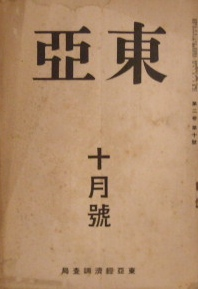
\includegraphics[scale=.5]{a20130223ThePoliticalPhilosophyofConfucianism-img001.jpg} 
\end{wrapfigure}

Now, Confucianism teaches that he who accords to Nature knoweth the Way. Mencius says that ``you must possess the five virtues yourself and extinguish your selfish nature", and this means the same thing. The autonomy of morality, which Kant outlined so carefully with his utterly precise logic, was not a unique discovery of the German philosophers. The Confucians rapidly grasped this truth based on their depth of experience. For example, Mencius' Four Sprouts are none other than a study of the foundations of human morality. What he calls a ``Sprout" is a ``natural foundation" from which morality can be grown. And so, in Confucianism, to work for ethical completeness is called development, or self-growth, or self-discipline. This capacity is inherent in oneself–he who possesses infinite possibilities for future action must start with an education in what is good. Therefore, the Tao as it pertains to Heaven, Earth, and Man first and foremost is something that should be realized through growing the natural foundations of morality in the self.

What is Heaven? Heaven is the origin of our existence. Most directly, this is our parents, and above them is our kin and ancestors. The origin of our ancestors is in the race, and the origin of that is in the universe. The correct relation to hold towards Heaven, that is to say, ``religion", is called in Confucianism Honor. This means growing and refining our essential human feelings of reverence and respect.

What is Earth? It is Nature as regarded by the mind. The most personal encounter we have with this is through our physical bodies, as well as the accompanying feelings of desire in our minds, as well as the external changes that these desires demand. The correct relation to hold towards Earth, meaning first the establishment of control over one's mind with regards to nature, and second the unification of one's attitudes, which may narrowly be called ``morality", is called in Confucianism Right. This means disciplining and training the essential human sense of shame, so that we will face towards Heaven unashamed and have good expectations for our life on Earth.

What is Man? Men are the individuals of good character whom you value equally with yourself. A well-bred man reasons with logic and acts with morality. Using logic, he understands the limitless possibilities of the complete knowledge of the universe, and thus is endowed with infinite possibility to realize in our lives, according to our intentions, the meaning of all things that it is possible to know. This personal limitlessness is called in Confucianism ``natural intellect, natural ability". Therefore, the proper relationship towards Man is to constantly develop the capacities of our natural intellect and ability, to our mutual benefit. Saying that this is realized through a purification of our natural tendency for sympathy and sentiment, Confucianism calls this Virtue. However, the collective effort to develop many intellects and abilities according to the parts of each and every life of many human beings in community is usually called politics. That is to say, the term politics is nothing other than an attempt to objectivize, or systematize Virtue.

Confucianism is therefore a Tradition that clarifies the three interests of religion, morality, and politics. Rather than breaking up these three ideas into separate fields of specialization, it understands them to interoperate as a single whole, and endeavors to eluciate the ``Tao" as a principle for all human life which contains all three. This is a point which has caused much outside confusion about the nature of Confucianism. One [Western Orientalist] will claim that Confucianism is a moral teaching, another will claim it chiefly conveys information about government, while still another lists it among the world's religions, but all their interpretation began from this source. For example, one Prof. Douglas calls Confucius' teaching nothing more than ``a plain, matter-of-fact system of morality". But Confucianism is not a religion in the Western conception of the thing, nor is it ethics or political science. Confucianism is not a single one of those, but is indeed all of them at once. Recognizing this as an internal structure, we can resolve the external confusion: this is a Tradition which we will understand nothing of from a Western perspective.\footnote{A postwar revision, and further thoughts on the concept of ``religion", can be found on my website: \url{http://avery.morrow.name/blog/2013/02/the-tao-of-the-east-and-the-last-samurais-testament/} }

\begin{quotex}
Here, \textbf{OKAWA Shumei} begins to make his departure from the basic principles of Western political thought obvious, deploying a slightly Hobbesian character from the 3rd century B.C., and demonstrating his Confucian orthodoxy. It is interesting to consider this contrast of rules vs. rulers in the modern cases of businesses, schools, etc.

\end{quotex}
The political thought of Confucianism is built on top of this fundamental spirit. Accordingly, most orthodox Confucianists could not be made to target politics as a thing standing alone and separated from religion and morality. The personal training for politicians, given names like ``study of ethical use of authority" and ``way to a virtuous nation", was never a thing separated [from the basic texts and principles]. According to Confucianism, as politics is the embodiment or systematization of Virtue, so the most essential basic requirement of the politician is to amass much virtue in their hearts. So most Confucian political works are expositions of knowledge intended for the ruler or politician. That is, to explain to the ruler the correct attitude for his heart, and how to attain virtue and compassion in his heart, is the basic method of Confucian political science.

For example, the Han \emph{Treatise on Punishment and Law} states, ``An ancient saying has it that even if the whole room has been eating and drinking, if there is one person crying to herself in the corner, no one in the room can enjoy themselves. And for a ruler, just like the case of that room, if even one person in his realm is treated unfairly, one's heart takes pity." An edict of Emperor Zhang of Han states, ``The sovereign must treat the people as if he were their father or mother, answering hardships with love, teaching loyalty and virtue, and administering appropriate punishment." Throughout the \emph{Shi Jing}, the ruler is portrayed as the mother or father of the people.

Indeed, as a consequence of understanding politics as the embodiment of Virtue in this way, the political ideal of Confucianism can be summarized in a phrase as ``domestic tranquility". Domestic tranquility means that for all of the people that exist in a nation, throughout their lives, negatively speaking they meet with no obstacle, or positively speaking, they are able to fulfill their respective functions. Nevertheless, regardless of the institution or organization, the expectation of true domestic tranquility does not mean that it is rigidly enclosed by [bureaucratic] considerations. At the top of Xunzi's thesis on sovereignty, he uses the phrase, ``\textbf{Rulers, Not Rules}``. And this phrase is the single clearest declaration of Confucian philosophy as it relates to systems and organizations, meaning that the aim of politics is not the \emph{rules}, but the \emph{character of the politicians}. Indeed, Xunzi's full statement is as follows:

\begin{quotationx}
Not a country in disorder, but a leader in disorder; not rules of order, but rulers in order. The methods of the archer Yi are not lost, yet such an archer does not appear generation after generation. The laws of King Yu of Xia still exist, yet the Xia could not continue their rule. Thus, laws cannot stand alone. Categories cannot apply themselves. If there are good men then the nation will survive. If there are no good men then it will be lost. Laws are the sprouts of order, and the man of virtue is the field in which that order grows. If men were virtuous enough we could even do without laws, but if no man is virtuous, no laws will suffice to save us, and we will fall into disorder. One who can simply count off the laws without knowing the Right behind them, no matter how learned you might call him, if he is given authority disorder will result. Therefore, a good king goes swiftly in search of good men, while a bad king seeks out power.

You ask how to rule a nation. You should first ask how to discipline yourself, before you can run a nation. The sovereign rules, and with his right rule comes right views. The sovereign is a bathtub, and his people are like the water. Water follows the shape of the tub. If he is a round tub, they will be round, and if he is a square tub, they will be square. It does not matter if it is the sovereign's edicts or his mere whims. King Zhuang of Chu preferred slender bodies, so there was starvation at court. If you must ask how to discipline yourself, you do not yet know how to rule your nation.
\end{quotationx}

Mencius means the same thing when he says frankly that ``without men of virtue, there can be no rule", and a famous chapter from Confucius' \emph{Doctrine of the Mean} goes, ``The government of Wen and Wu is recorded on tablets. Let there be such men and the government will thrive; but without such men, the government decays. With men who heed the Tao, government flourishes, just as agriculture flourishes when the Tao of the Earth is heeded; indeed, government matures just as reeds shoot forth from the soil," expressing the same idea.

The theory being expounded in \emph{Doctrine of the Mean} is as follows. An ideal government existed in the time of Kings Wen and Wu, which can be verified through various documents. People like them can govern splendidly, but without people like them, good governments can crumble. If good people are promoted to government, it is like plants growing from rich soil, and the results will come quickly. The rise and fall of individual politicians has immediate consequences in politics, just as a sudden change in soil quality has an immediate influence on the plant. Regardless of political system, our politics depends on the character of the people in it. And the type of people who will be appointed depends solely on the character of the ruler. Moral principles must be protected to establish good character. And virtuous love must be cultivated to possess those moral principles.

\begin{quotex}
Translation notes: The term ``man of virtue" means an educated elite, and is similar to how Julius Evola employs the term ``Aryan".

The Confucius translation is adopted from several English sources, rather than Okawa's incomprehensible late medieval transliteration (which he re-translates in the next paragraph). The first fourth of the Xunzi translation, about the archers and the Xia, is derived from Kurtis Hagen, \emph{The Philosophy of Xunzi}, Open Court Press, 2007. The rest is original and somewhat loose, but I swear to God he really does say the sovereign is like a bathtub.

\end{quotex}

\hfill

\begin{quotex}
Now, \textbf{OKAWA Shumei} takes out the big guns, attacking the founder of Legalism as impeding the cultivation of virtue, and by implication Western political theories which aim for the same legalistic goal. What the reader might not realize is that in denouncing Han Fei, who lived in the 3rd century B.C. and had an influence on all Far Eastern political thought thereafter, Okawa is arguing for a return to a very ancient ideal indeed. When a group of ultra-nationalists tried to overthrow the constitutional monarchy of Japan in the name of direct Imperial rule, Okawa was sent to prison for five years for providing the theoretical principles for such a political concept.

\end{quotex}

This concept, the greatest conceivable system to realize human ideals in an actual nation, comes into obvious opposition with the political philosophy of the West, which attempts to induce people to march automatically, so to speak, towards progress and perfection. Western political thought, in the words of Xunzi, has ``rules, but no rulers"; that is to say, it values creating good ``laws" over creating good ``men". Even in China, some sages like Shen Dao, Yin Wen, and Han Fei value law over men in their writings. Han Fei, especially, fiercely attacks the idea of ``rulers without rules" in one of the chapters of his book, and devotes himself to organizational structure. What he claims is that waiting for a man of virtue to appear is like a hungry man refusing to eat for a fortnight while he waits for a prime rib to arrive; the poor soul will simply starve to death.

His argument goes like this: Even with a total disinterest in organizational structure, a nation can be ruled by the likes of an Emperor Yao. And even with the finest organizational structure, a nation ruled by a tyrant would quickly dissolve into chaos. But a great Emperor Yao or a tyrannical King Jie will appear only once in a thousand years. Most rulers are neither Yao nor Jie. To create a nation that can be ruled by ordinary rulers, we must create the appropriate institutions. Creating people rather than rules creates a nation that can only be ruled once in a millennia, while creating rules for people will make a nation that is only disrupted once in a millennia.

Han Fei declares this to be a truth that is difficult to deny, and indeed, if we place our faith completely in the personality of a ruler, the result will be as Han Fei describes. But in Confucianism, even if there have been some who put an undue emphasis on it, there has been no one who disputes the meaning and value of ``laws". Actually, in the \emph{Doctrine of the Mean}, the three major functions of the ruler are piety, governance, and intellect. Piety implies both religious courtesies and moral customs, while governance means legal and political systems, and intellect refers to literacy. Without grasping the aforementioned three things, one cannot be a ruler in either name or reality. Even the most earnest abstract desire for a ``domestic tranquility", without institutions in place to ensure true domestic tranquility, we would not expect anyone to call someone a real politician. Mencius says, ``Mere good intentions do not build a government, nor do mere laws." The ``mere" here means subjective, or abstract. Confucianism, therefore, does not at all ignore structure, but recognizes that spiritual development must be esteemed over mere structure.

The success of all systems is, without a doubt, the result of a success of the human spirit. Therefore the true meaning of a structure cannot be grasped by the people who join into that structure if they lack a spiritual foundation. It becomes accordingly difficult to maintain it effectively. A genius who knows all 3,000 rules of etiquette and 300 marks of majesty, if he fails to grasp the true meaning of piety, will simply fall into useless, machine-like imitations. And in order to grasp the true meaning of piety, we need true hearts and good faith. This is why Lu Jiuyuan said, ``If we fail to overcome our own selfishness, it will be difficult for us to know virtue. And without a full knowledge of virtue, we will know not what rules and regulations are for."

\begin{quotex}
I continue directly into the conclusion. Hopefully all the readers of this blog will be quite gratified to see this independent manifestation of the Traditional principles.

\end{quotex}


Now, in Confucianism, there is a strong emphasis on ``love for relatives", or ``veneration for noble deeds" as a principle for social life. In the \emph{Doctrine of the Mean}, Confucius teaches: ``The humanity of virtuous behavior is made evident in the case of love for relatives. The ability of righteousness to set things straight is made evident when we honor noble men. The decreasing measures of the love due to relatives, and the steps in the honor due to the worthy, are produced by the principle of propriety." The implication of this passage is, approximately, as follows. Virtuous love binds people together, and its most striking manifestation is in our natural affection for our parents and kin. In contrast, justice is a type of discrimination. Its most striking manifestation is when we naturally hold some sense of respect towards noble men, that is to say, those whose moral values tower above all of us.

Nevertheless, we do not love all of our relatives equally. Even if the original source of virtuous love is an indiscriminate, equal substance, it is utterly unforgivable for its manifestation to be uniform in nature. Our reverence towards ethical exemplars, too, is of the same nature. In the manifestation of virtuous love and reverence, the attempts to confer a correct order are the grounds that generate the various forms and systems of social life. It is an indispensable condition for a Confucian social order that social inequalities are generated from a correct moral foundation.

Both love for relatives and veneration for noble deeds are called much more simply ``filial piety" or ``respect for the elders". One of the first statements in the \emph{Analects} reads, ``A youth should be filial at home, and, when abroad, respectful to his elders." The model for household life necessitates recognizing the position of parents, and each sibling among the children disposes of his ``self" and faithfully works for the sake of his family and clan, continuously realizing an order of being. Honoring virtue, similarly, underlies the model for national life, and Confucius teaches that the exercise of authority both large and small necessitates a shared concept of virtue, which people must entrust to the statesmen, abandoning their ``self" interests and faithfully obeying the authority of the state.

Therefore, the duties of the men of noble birth in China were not rule of the country–personal oversight as administrators–in the usual sense, but were actually the promotion of able men to wield authority in roles both great and small. Therefore, it is said that ``if we hasten to get the right men, the self is checked and the nation is put in order, the merits are great and one's name is celebrated, and one is worthy of being called a sovereign. If we do not hasten to get the right men, but instead focus on getting the labor first, then people will work for their own purposes and divide the nation, merit is abandoned and one's name is besmirched, and the very soil and grain of the nation will certainly be endangered. The worthy sovereign seeks out the men and, having found them, may rest."

``If the people be led by laws, and uniformity sought to be given them by punishments, they will try to avoid the punishment, but have no sense of shame. If they be led by virtue, and uniformity sought to be given them by the rules of propriety, they will have the sense of shame, and moreover will become good." This is a famous saying of the \emph{Analects}, and a summary of the essential spirit of Confucian political philosophy. […] And there is one point on which Confucianists and Legalists agree. Namely: what constitutes an upright citizen, in other words the attempt to forge a tempered and cultivated political individual, is a separate matter from the legal system, in other words the attempt to establish a systematized nation-state. Again, in other words, while Legalism insists on the strictly impartial nature of legislation, Confucianism remains the first principle at the root of litigation [because the goodness of a person is based in Confucian values].

In this way the political doctrine of Confucianism is generally not called one of constitutionalism, but is rather rite-ism, and the relation between laws and rites is perfectly encapsulated by Liang Qichao, who said that ``laws treat the symptoms, but rites are preventative health." According to Confucian political science, the sole foundation of good government is indeed cultivation of culture and learning: ``right learning brings good customs, and good customs bring good government."

The political thought of Confucianism, as clearly indicated by all the histories, was never implemented closely in China. The finest implementation of it up until now was in our own nation's Tokugawa period. The shape of our nation in that era rivals and even exceeds that of China's Spring and Autumn period, showing that the political ability of the Japanese far outstrips that of Han Chinese. The China of the Spring and Autumn Period was not much different from the old shogunate in population, area, or feudal development. Accordingly, the political ideals of Confucius and Mencius, although meant for a united China, became much more relevant in our own country, and our political ability was not just a realization of those ideals but a superior realization to that of China.

Thus in the Tokugawa period, the ideal that made the sovereign parent to the nation became ingrained in the hearts of the provincial lords, and when one province achieved a temporary state of good leadership, other provinces felt a need to compete [as in sibling rivalry] and strained to achieve the same standard, creating a splendid government. That China later descended into pandemonium and confusion despite its cultivation of Confucianism is not due to any insufficiency in Confucianism itself, but the fault lies in the political incompetence of the Han.

\begin{quotex}
The pointedness of this last paragraph lies in the fact that Okawa has just made use of brilliant reformists like Liang Qichao (1873-1929), but unlike their Japanese counterparts, the Chinese reformists failed to rebuild and modernize China.

All credit for the production of this translation lies with the Okawa Shumei Study Group which made these materials available. All fault for the numerous translation errors and misrepresentations lies with me.

\end{quotex}


\flrightit{Posted on 2013-02-21 by Avery Morrow }

\begin{center}* * *\end{center}

\begin{footnotesize}\begin{sffamily}



\texttt{Lemonheadz on 2013-02-22 at 00:28 said: }

Did Okawa have any contact with Guénon or his school of thought?


\hfill

\texttt{Avery Morrow on 2013-02-22 at 00:35 said: }

Okawa unfortunately seems to have missed out on Guénon and his school. His leanings in that direction, though, are demonstrated by a book he translated for a man named Paul Antoine Richard, the husband of Sri Aurobindo's spiritual successor ``The Mother". Richard's book is indistinguishable from Aldous Huxley's The Perennial Philosophy which was written 2 or 3 years later. After long conversations with Richard, Okawa became a big fan of Sri Aurobindo despite a lack of thorough reading into his philosophy.


\hfill

\texttt{Jason-Adam on 2013-02-22 at 17:58 said: }

Honour also consists in admitting your sources. You don't learn from China and Korea and then take their women as your sex slaves and their men as forced labour. Japan behaved with great dishonour during WW2 and was punished by Heaven for it.

I strongly advise that in studying the Far Eastern form of the tradition, we should avoid the Japanese derivative forms and look to the roots in China and Korea…..

For the record let me also say that the Koreans are a much stronger martial people than the Japs, they beat the French and Americans in the XIXth century and the Japs many times over the centuries, last time being WW2.

I am presently preparing to be initiated into a Korean order…..


\hfill

\texttt{Avery Morrow on 2013-02-22 at 21:24 said: }

I can't really comment on your principle that the truthfulness of a text can be judged by the circumstances its author lived in, nor that military defeat is a sign of martial strength, but I feel obliged to at least correct your inaccurate claim of ``sex slavery"; not only was no slavery involved in Japan's military brothel system, but it was taken over by the Americans and used in the Korean War, and a similar system was set up by the Americans in Vietnam, purchasing women from impoverished Vietnamese families. Please see this academic summary of research into the subject.


\hfill

\texttt{Janus on 2013-02-23 at 17:37 said: }

I must disagree here…the extent to which a woman in poverty can really be said to be ``willing" in her prostitution is highly debatable. The amount of freedom she really had once in the hands of soldiers, Japanese or American, even more so.


\hfill

\texttt{Janus on 2013-02-23 at 17:42 said: }

The tripartite division of Confucianism presented here is interesting, but does it not focus more on the cult of the ancestors than the cult to Divinity? Or is this Divinity contained in the ``universe" which births the race, ancestors and parents?

The acknowledgement of Confucianism as an organic ``living" practice, rather than just a philosophy is essential and something I am glad to see here. The western insistence on dividing learning, work, life, religion, and so on is a major sign of its degeneration. His comment on the western perspective is spot on, although I must agree with doubts expressed about using the Japanese rather than original Chinese perspective, particularly one coming from the Imperial era of the 20th century rather than pre-Meiji Ishin.


\hfill

\texttt{Jason-Adam on 2013-02-23 at 17:57 said: }

It's a tricky matter. My grandfather was a rikuguntaisa in the Japanese army during the Greater East Asia War but after visiting Korea I feel as if I need to make penance for his misdeeds.


\hfill

\texttt{Avery Morrow on 2013-02-24 at 06:43 said: }

This is too late at this point, but I'm sorry for my rather accusatory and grumpy comment. I thought about it a lot today, and I am certain my attitude stems directly from reading too many high-tempered Internet arguments.


\hfill

\texttt{Jason-Adam on 2013-02-28 at 21:53 said: }

The author shows his racism by blaming the problems of China on racial defects and not on failures of character, failures that afflict men in all nation, and have made Japan a cultural and political colony of America since 1945.

In fact, China under the Qing dynasty was a quite stable and functional regime until the British imposed opium addiction on the Chinese people.

I see a contradiction in that the author praises Edo period Japan, which was a peaceful, feudal, and autarchical era yet he supported ultra-nationalism which was more like Fascism in supporting an expansionist centralised state under the dictatorial rule of the Mikado who was no longer the spiritual figurehead he was under the shogunate but an actual Bonaparte-type sovereign under this sytem (I'm thinking also of Ikkai Kitta)


\hfill

\texttt{Avery Morrow on 2013-02-28 at 22:01 said: }

You forget that China was not the only East Asian nation struggling with Western interference; Japan was also thrown into crisis by Western temporal power, and its response was quite different from China, while its blazing fast modernization and militarization was due in large part to the efforts of Emperor Meiji himself.

Okawa witnessed the failure of both China and Korea to adapt in his own lifetime, and the near subjugation of both nations by the West; he has ample reason for his patriotic attitude. I would wager that he is actually a more appealing figure than Evola, who discarded sentimental ties to family and nation.


\hfill

\texttt{Jason-Adam on 2013-03-01 at 18:01 said: }

Modernisation……that's the problem…….in order to fight the West, Japan became a western power. 

China and Korea failed, yes, though in the Korean case the failure is arguable as I can attest to the survival of Korean tradition through my own studies in that nation. But the failure is simply that of traditional falling to modern which is not a good thing in my book, as I'm a supporter of the old ways.

Asian patriotism like any patriotism is a good thing but not when it becomes a tool for colonialism – if Japan had led Asia against the West he'd have been heroic but instead the Japs decided to just enslave fellow Asians in Manchuria, Korea, and China.

PS – the US tried to open up Korea in 1866 the same way they did with Japan in 1853 but that time the Koreans won and the big noses came home dead…….

I prefer Evola's attitude of placing principles above false realities……he saw the true state of his Italy and did not fail to expose it…..


\hfill

\texttt{Avery Morrow on 2013-03-01 at 18:44 said: }

To try to drag the discussion back to the actual nature of this essay, I don't think Evola's political vision is that far from Okawa's, except that the situation in Italy ensured that Evola could never dream of implementing a Traditional government, whereas Okawa had many adepts hoping to do just that.


\hfill

\texttt{Jason-Adam on 2013-03-01 at 23:13 said: }

I hope I am discussing Okawa's essay here when I raise issue with the fact that he claims China never properly implemented Confucianism, I would like to know that if he is correct, then how would he describe the ruling ideology of the Chinese empire from the Han dynasty (200 BC) to the end of the Qing (1912 not counting its revival in Manchukuo, 1930s)?

The difference I am seeing between Okawa and Evola, correct me if I am in error, is that whereas Evola wanted the unification of Europe under a supranational Emperor that transcended nationalisms, Okawa believes Japanese nationalism can unify Asia under Japanese domination ?


\hfill

\texttt{Janus on 2013-03-02 at 00:31 said: }

Fascinating piece, though I must too express my disappointment at his ease in asserting that there was some racial flaw in the Han which caused the decline in China, especially when he mentions periods in Chinese history when righteous rulers came to power. 

I'm also glad to see that he discussed Legalism, the philosophy predominant in influence in China today, especially on the political stage, and that he can do so without quickly dismissing it. Political ideas and movements are revealed for what they are without men and women of quality making up the numbers: utopian ideals at most, and farces leading to tyranny at worst (see the Conservative revolutionaries, who allowed their ideas to be hijacked by those for whom Aryans were a mere biological race). It is essential to make good laws in the State, but even more to realize that they are there to craft good human beings. This is the most radical assertion one can make in the political and social realm, and a dangerous one which can lead to tyranny if there is no direct and positive correlation between position in the hierarchy and standard of character and accountability. 

I heard two quotes in a performance of the Trial of Socrates which I think beautifully encapsulates the Confucian view in a democratic context: ``In a democracy, you're only asked to do two things: obey the law, and try to change it if you think it's wrong." and ``You accepted the constraints of the law every time you accepted our protection and did not speak in the Assembly in order to craft the best laws possible." Without good and just men, there is no good and just order.


\hfill

\texttt{Avery Morrow on 2013-03-02 at 05:09 said: }

What was actually implemented from 200 BC to the 1930s was Legalism, which was argued in this essay to be a distortion of the original tradition. (In the same way that the Christian medieval world was a distortion of the Roman imperium? Maybe? Hmm.)

That's a great question. I honestly don't think Okawa had such a naively imperialist view, but his geopolitical analyses are yet on my to-read list, and if I translate anything else by him on Gornahoor I will mention what I learn.


\hfill

\texttt{Jason-Adam on 2013-03-02 at 17:32 said: }

@ Avery

It would be good to read more of Okawa's ideas, as the close relationship between geopolitics and tradition is something I feel Guenon and Evola did not see…………

It's very interesting, the subject of Legalism, I remember reading once someone tried to argue that Maoism is actually derivative of Han Fei Zi, it is true that to some degree Mao admired Qin Shi Huang, the persecutor of the Confucians…… 

In a western context, do you think Plato is closer to Confucius or Han Fei ? The fact that he wrote a book of Laws seems to indicate P. thought he could legislate for a state beyond the capabilities of individual men ?


\hfill

\texttt{Avery Morrow on 2013-03-02 at 18:35 said: }

Just as a particular example, I think Plato's belief in the communal upbringing of children puts him squarely on the side of a Legalist legislating morality. That's not to say this idea is horribly dangerous, since Israel's kibbutzim implemented something like it and did not end in disaster. Nor is Legalism anti-Traditional; the early modern period was full of such attempts to preserve exoteric manifestations by putting them into law.

But the Roman imperium was not characterized by a huge list of laws and a great bureaucracy maintaining them. People's instincts for things like raising their own families were considered to be basically good, and only needed cultivation through education. I think Okawa and Evola are both right to claim that in the ``world of Tradition", Law is only expressed through obedience to the Principles, which are self-explanatory and within every human heart.


\hfill

\texttt{Avery Morrow on 2013-03-02 at 23:28 said: }

One last note: if anyone would like to flesh out their knowledge of Xunzi I found a Ph.D. thesis which supports Okawa's thesis that Xunzi defended real Confucianism from Legalism, actually closely imitating the conclusion that Confucianism supports the concept of laws but Legalism turns this into an obsession.

http://scholarspace.manoa.hawaii.edu/handle/10125/3023

Excerpt: ``While Confucian constructivism can support a theory of universal human rights, if it is to remain Confucian, it would not emphasize this because Confucianism perceives reasons not to foster a strong rights culture. Rights are viewed as legalistic mechanisms which, if over-emphasized, can erode informal mechanisms such as Ii (ritual propriety), the maintenance of which is considered critical to maintaining a healthy society. Citing several passages from the Xunzi, along with other Confucian texts, Ch'ii T'ung-Tsu concludes: `Confucians firmly believed that … The order or disorder of a state … depends completely upon the maintenance or the decay of li' (Ch'u, p. 241). To the degree rights seem to undermine rites, they will likely continue to be resisted."


\hfill

\texttt{Jason-Adam on 2013-03-02 at 23:57 said: }

Avery, so in your view one can be a Confucian or a Legalist and still be Traditional ?

Would you define the Torah or the Shariah as versions of Legalist thought ?

I wonder if the purpose of Confucianism and Legalism are for different ages, the age of Yao and Shun compared to our time from a Hindu perspective is different points and the cycle and different styles of governance perhaps may be required ?


\hfill

\texttt{Avery Morrow on 2013-03-03 at 00:24 said: }

I would agree that Confucianism and Legalism are both Traditional and suited different ages, since this is grounded in historical fact as well. It's also obvious that rabbinic halakah did not exist when Israel was a kingdom (the Torah and Talmud are not solely legal texts). But shariah just as clearly comes from the ``seal of the Prophets" himself, befitting the 8th century AD.

This exchange has made me wonder much more seriously whether a ``return to Confucianism" would approximate a Protestant desire for the simplicity of the earliest sources without the awareness that we are living in a degenerate age. Evola, of course, would disagree, and there are plenty of medieval texts that assert that Confucius takes primacy over his commentators, but I would like to see what Schuon says on the matter.


\end{sffamily}\end{footnotesize}


\chapter{The Ancient City. Greek and Roman civilizations}
\section{Race and the Myth of the Origins of Rome I}

\begin{quotationx}
This essay by \textbf{Julius Evola} was originally published in the journal \emph{La Difesa della Razza}.

In the context of the recent series of posts, this can be understood as the ``Noble Lie" about the birth of Rome. From the point of view of profane history, these myths are simply superstitions. Evola, on the other hand, drawing on Vico, Bachofen, Guenon, \emph{inter alios}, views such symbols, myths, and legends as witnesses to the inner spirit of a people, which cannot be grasped simply in the accumulation of historical facts. Logically, this technique leads him to move beyond the merely physical and zoological understanding of race to the notion of the races of the soul and of the spirit. (This is a reformulation of the Rosicrucian notions of the folk soul and folk spirit.)

In this first part, Evola brings to light two aspects of the myth. First is the idea that the founder was born from the union of a god with a mortal woman. The god confers spiritual qualities on the founder. In this case, Mars, as the god-father of Romulus and Remus, is the spirit of warrior virility, not just on the twins, but on the entire city.

The second aspect is being saved from the Tiber as infants. For Evola, this represents the hero, the seer, etc., men above the flow of time.

The defect in Evola's methodology is that he is left in the same position as the profane historian: the third person perspective. Although he sees more deeply, he is still an outsider and does not participate in the myth. So, yes, for him, too, it is a Noble Lie. For the Romans, Mars was a living being, not some abstract force, and the story of their miraculous rescue from the Tiber was considered history, not legend.

Although we can get some idea of the spirituality and mentality of the Romans from Evola's analysis, a scholarly discussion cannot lead us to that same state. For that, the method of Hermetic meditation described by \textbf{Valentin Tomberg} is much more helpful\footnote{\url{https://www.gornahoor.net/?p=898}}. This is a lesson for those hoping to establish a new regime somewhere, sometime: they must create a noble lie that is also a spiritual truth. 

\end{quotationx}
In his \emph{Life of Romulus} (I,8), \textbf{Plutarch} writes:

\begin{quotex}
Rome would not have risen to such power had it not had, in any way, a divine origin, such as to offer to the eyes of men something great and inexplicable. 

\end{quotex}
\textbf{Cicero} repeats the same thing (Nat. Deor. II,3,8) and considered (Har. Resp., IX, 19) the Roman civilization as that which through sacred knowledge ``surpassed every other people and nation": \emph{omnes gentes nationesque superavivums}. Sallust called the ancient Romans \emph{religiosissimi mortales} [the most religious mortals].

On the other hand, in our day all of that is fantasy or superstition for many ``serious" persons and many ``critical" minds. The ``facts" are the only things that count for them. The mythical traditions of the ancients have no value, or they have it only insofar as it is supposed that, here and there, they are confused reflections of real events, that is to say, tangibly historical. There is, in that, a fundamental misunderstanding that was already denounced, to a certain degree by our \textbf{Giambattista Vico}, then by Schelling, still more recently by Bachofen and, finally, by the most recent school of the metaphysical interpretation of myth, and by those little known today (Guenon, W. R. Otto, Altheim, Kerenyi, etc.). According to all these writers, the mystical traditions are neither arbitrary creations more or less on the poetic and fantastic plane, nor deformations and transpositions of historical elements. Especially in regard to origins, it was correctly pointed out that symbols and legends,

\begin{quotex}
if only in a dramatized form, represent actually and truly the history of the beginnings of a nation, but not the history of events occurring materially on earth, but rather of spiritual processes that have given birth to a new people alongside other people although different in culture and civilization: history, so to say, of its prenatal period.

Legend and history are tightly connected; the former proceeds through interiorization and is dispersed through images, while the latter proceeds through exteriorization as facts and events. These images are the result of formative living forces, facts are organized by the human thought. In legends one is transported by formative forces; in the other, there is premeditated organization of facts. But the legend is the invisible part and root of history; it is not poetry, rather it is a reality much vaster than history itself. The threads of the destiny of a people that unravel visibly in the most various ways in their historical development, go back to the impulses, to the creative spheres, to which the heroes of its legends are connected. 

\end{quotex}
In a particular way, \textbf{Bachofen} revealed that even at the point in which evidence, by being recognized as a myth, came to be rejected by profane history, even when it is a positive witness to the spirit of a people.

In that way, a study of mythical traditions, using new criteria, can lead us to interesting conclusions from the point of view of a theory of race that is not defined by the material aspects of the issues, but also addresses the inner reality of race.

On the occasion of the current anniversary of the Birth of Rome, we want to illustrate this interpretative method, applying it precisely to the exegesis of the myth of our origins. The legends related to the birth of Rome concentrate such a quantity of sensitive elements based on general meanings of civilizations and mythologies of Aryan peoples, that a special work would be necessary to analyze them and clarify them adequately. Therefore, we will point out here only the most notable themes, among which are: the miraculous birth, the theme of being ``saved by the waters", the ``wolf", the ``tree", the rival pair of twins.

The myth of the union of a god with a mortal woman, in the present case, of Mars with Rhea Silvia, from which union Romulus and Remus were born, recurs in almost all traditions in regard to the birth of ``divine heroes". Zeus and Leto gave birth to Apollo, Zeus and Alcmene to Hercules, Heracles being the symbolic hero of the Doric-Achaean Aryan peoples, and Apollo having a connection with the land of the Hyperboreans and with the primordial Nordic-Aryan races. An analogous origin, in properly Germanic traditions, is attributed to the heroic peoples of the Volsungs, to which Siegfried belongs.

In the ancient royal Egyptian tradition — whose remote origin can with good reason also be considered to be Aryan, Atlantic-Occidental — every sovereign is thought to have been begotten by a god uniting with the queen: this tradition in which the hidden meaning of the myth comes to the fore, inasmuch as a miraculous birth without the help of a man, of a human father, was imagined. Since the queen had her consort, the idea that her son was conceived by a god, being awakened to life by her husband, could only indicate that he, not in his moral part, but so to say, in that eternal and ``divinatory" part, had to be thought of as a type of incarnation of a decisive supernatural element that came to confer a royal dignity on him.

In the case of Rome, therefore, Mars is such an element from above, that is, the divine representation of the principle of warrior virility. Such a force stands therefore at the origins of the Eternal City and at the basis of its secret origin, veiled by the legend: so that in some traditions from the era of the Roman Republic itself, it will be directly conceived as the ``son" of Mars. And this ``Mars" force is associated with those who may be the guardians of the sacred flame of life; symbolically: with a vestal (Rhea Silvia).

\begin{wrapfigure}{rt}{.4\textwidth}
 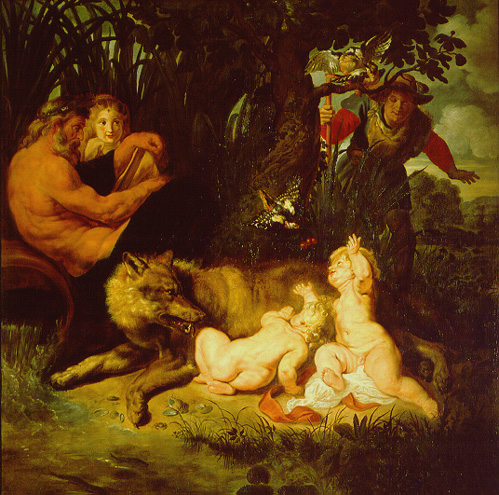
\includegraphics[scale=.3]{a20141211RaceandtheMythoftheOriginsofRome-img001.jpg} 
\end{wrapfigure}

The twins Romulus and Remus are abandoned to the waters and are saved from the waters. Here again is a symbolic theme recurring in many traditions: Moses is saved from the waters, the Indo-Aryan hero Karna is left in a basket in the river and is saved from the waters, and so on. But the symbol contained in the most ancient Aryan tradition is especially important, i.e., the Vedic tradition, in which ascetics are depicted as ``supreme natures who stand on the waters". Analogous explanations and, therefore, the hidden meaning of such a symbol, can be clarified as follows: the waters have traditionally always depicted the current of time, i.e., the basic element of mortal, unstable, contingent, passionate, fleeting life. The weak man is taken from the waters and carried from the waters. The seer or hero, the ascetic or the prophet is saved from the waters, or is capable of standing on the waters, or of not sinking in the waters. Hence, in the myth of the origins of Rome this symbol must again characterize the ``divine" element of the founders of Rome, their, so to speak, supernatural dignity.



\begin{quotex}
This is the second and concluding part of the essay by Julius Evola on the race and origins of Rome.

He points out the symbolism of fig tree, which was also the tree associated with the Buddha's awakening. The next symbol is the She-Wolf who suckles the twin babies. The wolf curiously has a dual symbolism: it can represent both the forces of light and the forces of darkness. This is often depicted as the battle between order, or Logos, with Chaos.

It is interesting to point out that the primal symbol of the wolf has been replaced in our time with the lap dog.

The spirit of Rome is exemplified by the manifestation ``of a principle of light and of order, of an ethic and a vision of life that is witness to the Aryan spirit". Here it is made clear that the Roman race is known through its spirit, not its genetics. So before constructing our Republic, it is necessary to describe that principle, ethic, and vision.

\end{quotex}
The twins find refuge near the fig tree [\emph{Ficus Ruminalis}] and are suckled by a She-wolf. The word Ruminal contains the idea of feeding: the quality of Ruminus, related to Jupiter, alluded to the quality of ``nourisher", of the ``god who gives nourishment" in the ancient Latin language. But this is the most elementary aspect of the symbol. In general, in the most ancient traditions of the Aryan races, the tree is the symbol of universal life, it is the tree of the world or the cosmic tree. If it is in form of a fig tree as it appears in the legend of Roman origins, precisely as a ``\emph{fico indico}" [Banyan tree] — the ashwattha tree — it is depicted as upside-down in the Indo-Aryan tradition to express that its roots are from above, in the ``heavens". The idea of a mystical food from the tree is a often recurring theme: the myth of Jason, Hercules, Odin, Gilgamesh, etc. Naturally, according to the races and their spirit, this then presents diverse variations. We know from the Hebraic myth that to pick and eat from the tree in order to make oneself like god is considered as the principle of guilt, abuse of power, and a curse. Things are conceived in a very different way in the myths of the Aryan races and even in the paleo-Chaldean myth of Gilgamesh. Also, in the legends of the Ghibelline Middle Ages, the heroic theme prevails and the tree often appears as that of the universal empire, reaching it in the symbolic lands of the mysterious Prester John means insuring the same dignity that the ancient Ario-Iranian rulers associated with the title of ``king of kings".

Returning to our main subject, in the myth of the twins at the origins of Rome, we therefore have the allusion to a supernatural food from the Tree — but also from the She-wolf. The symbol of the She-wolf, considered in its entirety and in all the stories that refer to it, has an ambiguous character. Lucian and Emperor Julian recall that, in the ancient world, on the basis of the phonetic resemblance between the two words, the idea of the wolf [\emph{lupo}] and of light [\emph{luce}] are often associated: \emph{lykos}, which in Greek means world, sound like \emph{lyke}, light. But there are also figurations of the wolf as a hellish animal, as a dark force. The Wolf thus appears to us in the double aspect, symbol of a ferocious and savage nature and also as the symbol of a luminous nature. This duality is verifiable, not only in Hellenic-Mediterranean prehistory, but also in the Celtic and Nordic. In fact, on the one hand in the Nordic-Celtic and Delphic cults the ``wolf" is connected to Apollo, i.e., to the Hyperborean, Nordic-Aryan god, simultaneously conceived as the solar god of the golden age and significantly associated by Virgil with Roman greatness. ``Sons of the wolf", on this basis, was a designation for warrior and heroic peoples of Nordic-Germanic origins, designations that persisted even to the epoch of the Goths and Nibelungs. Yet, on the other hand, in the Edda, the ``age of the Wolf" signifies a dark age, marking the epoch of the outbreak of savage and elementary forces, almost of the power of chaos, against the forces of the ``divine heroes", or Æsir.

Now we can certainly also relate this duality to the principle that, according to the legend of origins, ``fed" the two twins insofar as we see it reflected in their very nature, that is, in the antagonistic duality of Romulus and Remus, as related to us in the myth. As others already noticed, so also the theme of a single principle from which an antithesis is differentiated, whether depicted by the antagonism of two brothers of twins or, in general, of a couple, is found again in many traditions, and not rarely in respect to particularly significant moments for the origins of a given civilization, race, or religion. For example, we only recall that in the ancient Egyptian tradition Osiris and Set are two brothers of discord — sometimes conceived as twins—and one incarnates the luminous power of the sun, the other, a dark, ``infernal", principle, whose generation is called the ``sons of the impotent revolt". Does not something similar also show through perhaps in the Roman legend? Romulus is the one who marks the contour of the city as the meaning of a sacred rite and a principle of \emph{limit}—of order, of law—having received the right of putting his name to the city from the apparition of the solar number, of the \emph{twelve} vultures. Remus is instead the one who violates such a limit and is killed for this reason. One could say that the primordial force of Roman origins thus are differentiated and destroys the ``dark" powers that contained in themselves, affirms in its luminous aspect of order, Olympian domination, purified warrior force.

There have been attempts to see in the contrast between Romulus and Remus the reflection of the contrast between opposed Aryan racial forces, or of the Aryan type, and non-Aryan or pre-Aryan types. Research of this kind is without doubt interesting: problematic in its conclusions, if it intends to remain exclusively on the plane of material facts, or archeological and anthropological evidence. It has greater possibilities if it also penetrates the myth and legend in order to extract elements that integrate research in other domains. Naturally, in order to accomplish that, it also needs to resolve to outline general frameworks of various aspects of ancient Roman society, considering, for example, with various writers, somewhat probable that the social system of castes of ancient Rome had a racial substrate.

In this totality, it is interesting to examine the link between the two principles, whose symbolic figurations could well be Romulus and Remus, with the two hills Palatine and Aventine. The Palatine is, as we know, Romulus' hill and the Aventine is Remus'. Now, according to the ancient Italic tradition, on the Palatine, Hercules met the good king Evander (who significantly founded a temple of the goddess Victoria on the same Palatine hill) after having killed Cacus, son of the Pelasgian (pre-Aryan) god of the subterranean fire: and Hercules conquered and killed in Cacus' cave, \emph{located in the Aventine}, and erected an altar to the Olympic god, to whom he was allied according to the Hellenic myth. Researchers like Piganiol, are of the opinion that this duel between Hercules and Cacus — with the corresponding opposition of the Palatine and Aventine hills — could be a mythic transcription of the battle waged by peoples of opposing races.

The mythic legend of the origins of Rome is therefore saturated with deep meaning. The triumph of Romulus and the death of Remus is the key to the origin hidden in Romanity, and the first episode of a dramatic, outer and inner, spiritual, social and racial battle, in part known, in part still enclosed in symbols or in events not yet penetrated with respect to their most essential aspect, almost, we will say: with respect to the ``third dimension". Through this secular battle Rome rises gradually and asserts itself in the world as triumphal manifestations of a principle of light and of order, of an ethic and a vision of life that, in its original and uncorrupted forms, is witness to the Aryan spirit. And we know what it is, according to the most widespread tradition, the conclusion of the legend of origins: it is the apotheosis of Romulus, Romulus deified,

``he returned from the earth to heaven after his mortal part was destroyed by means of the dazzling fire."

So what has been treated is neither fantasy, nor poetry, nor rhetoric. Analogous explanations recur in the traditions of all peoples, according to a uniformity that should lead anyone to reflection. Also in regards to Romulus, the myth contains a faith and a spiritual certainty: it is the meaning of a reality that, freed from the person and symbol, was not once, but will always be, and will always be present, in its greatness beyond history, the race that knows how to recall the ``mystery".



\flrightit{Posted on 2014-12-08 by Aeneas }

\begin{center}* * *\end{center}

\begin{footnotesize}\begin{sffamily}



\texttt{Cologero on 2014-12-11 at 21:20 said: }

Tomberg quotes Hans Leisegang:

\begin{quotex}
Every myth expresses, in a form narrated for a particular case, an eternal idea which will be intuitively recognized by one who re-experiences the content of the myth. 

\end{quotex}
This is what Evola is getting at. So, of course, the myth ``contains" the eternal idea. Were it a simple reflection, then anyone could understand it. Rather, the idea is embedded, or hidden, in the myth, so it is discernible only to those who make the effort to re-experience it.


\hfill

\texttt{William Neville on 2014-12-13 at 01:51 said: }

Thank you for these translations, Cologero – this is valuable material.

It hadn't occurred to me before, but I wonder if Dante-specifically chose the She-Wolf as one of the beasts blocking the way out of the Dark Wood in the Divine Comedy as a reference to the She-Wolf in the story of Rome's founding. It would be interesting to meditate on and investigate.


\hfill


\hfill


\end{sffamily}\end{footnotesize}

\section{The Mystique of Race in Ancient Rome I}

\begin{quotex}
This essay by \textbf{Julius Evola}, which will appear in two parts, was originally published in the journal La Difesa della Razza.

By ``race", Evola means both something less and something more than is meant by the word today. ``Less" in the sense that a race refers to any group of people of a common stock or lineage. ``More" in the sense that he includes the transcendent, spiritual, and mystical aspect of race, not just biological or physiological characteristics. In this essay, he describes the mystical element of race in ancient Rome. A lineage was founded by a spiritual father, not necessarily the common biological ancestor; this father determined the cult, laws, and customs of his lineage.

Note on translation: I have left the words lares, manes, penates, genius (NOT a clever person), gens, and gente untranslated, following the model of \emph{The Ancient City} by \textbf{Fustel de Coulanges}. The interested reader should consult that work for the proper definitions.

Go to Part II $\Rightarrow $ 

\end{quotex}
The literature on racial theory has not failed to emphasize everything that shows the importance attributed to lineage, people, origin, and ancestry in ancient Romanity at that time, and has also conducted research to recover the Aryan or Nordic-Aryan element and type in Romanity and to follow its destiny. Because of the predominant interests in modern racial theory and in the very nature of its development, this research is therefore almost always focused on the basically exterior and subordinate elements: thus it remains on the level of ancient law and custom, on certain aristocratic traditions, on the direct or indirect evidence in respect to a give physical type and, somewhat less often, is conveyed in the field of the most noted and widespread certain cults and myths. It is curious that, as far as we know, it is instead almost systematically neglected a series of sources that, in regard to the higher aspects of the doctrine of race, present a special meaning and are richly documented. The reason for that is in the predominance of the prejudice—which we previously reported in this journal—to consider the whole of what in Roman antiquity had a super-rational and properly traditional character as fantasies, imaginations, superstitions, and finally, as something unserious and negligible. In this way a great part of the ancient Roman world still waits to be explored and this exploration, if conducted possessing the right principles and suitable qualification, is destined to yield valuable results, not just in regards to a spiritual and religious consciousness of the forces of the race.

The lares, penates, manes, genii familiari, the archeget heroes and so on are notions well known to anyone who has made even elementary studies of ancient Roman history. But known to what degree? Also, like the equivalents of dead and mute things that are conserved in museums, like the verbal residues of a world that is felt as foreign and ``dead", as much to leave us indifferent, at least, for whatever technical and academic reasons, they are not compelled to make special studies of sources and traditions, in place of mere culture, resulting in a worthy monograph. To integrate such signs, including pulling sufficient elements from them to make us understand the meaning and fundamental truths of ancient Roman and, in general, Ario-Mediter\-ranean, humanity is a task that, with very rare exceptions, is not at all felt. However, even by this we understand the most precise and significant racial profession of the faith of ancient Rome, not a ``philosophized" profession of faith restricted to any cultured circle, but alive and active in the most original, most widespread, most revered traditions.

The notions of lares, penates, genies, heroes, etc., are in good measure interdependent. In various ways, they all refer to the ancient Roman awareness of the mystical forces of blood and race, to the lineage, considered not only in its corporeal and biological aspects, but also in its ``metaphysical" and invisible, but not ``transcendent", aspects in the limited dualist meaning that has come to prevail for such terms. The single, atomic, deracinated individual does not exist. When he presumes to be a being in itself, he is deceived in the most pathetic way, because he cannot even name the last of the organic processes that condition his life and finite consciousness. The individual is part of a group, a folk, a gente. He is part of an organic unity, whose most immediate vehicle is blood, and is extended both in space and time. This unity is not ``naturalistic", is it not determined and called to life solely through natural, biological, and physiological processes. Such processes just constitute his exterior side, the necessary but not sufficient condition. There is a ``life" of life, a mystical force of blood and folk. It subsists beyond the forces of the life of the individuals that are dissolved in it at death or that are given by it through new birth: it is therefore a \emph{vitae mortisque locus} [a place of life and death]—a place that encompasses life and death and that for that very reason stands beyond both.

To maintain a living, continuous, and deep contact with this profound force of the race is the most direct and essential form of \emph{pietas}, religiosity, the basis and condition of every other, the principle canons of family laws are its consequences and applications, even in relation to the earth, that it itself—as the notion of the \emph{genius loci} shows—maintains mysterious and ``mystical" relations with the blood and the original strength of the people or \emph{gens} that possesses it and lives there. Looking toward the origins, there is the sense of a ``mystery"—there is the myth both of beings having come from above, and of men who transcended humanity, to loosen their life from their person and to thus constitute it as the superindividual force of a folk, of a lineage, of an ancestry that will see its origin in it. Ideally, there is a contact and a perfect match of the individual with this power, to be able to signify through it the apotheosis, i.e., the conquest of the privilege of immortality, and to confer on it the right to be considered even a ``son"—in a higher sense—of the being of the lineage, if even a type of new manifestation of this being itself.

This is the essence of the mystical-racial creed of ancient Ario-Mediterranean and, particularly, Roman, humanity. The significance that it gives to the race as spirit, beyond that of the body, is an irrefutable fact and constitutes the base of the belief of the entities indicated and of the meticulous worship that was dedicated to them. We will put forward some evidence that will also be valid to highlight further aspects of the central ideas we succinctly exposed.

According to a noted work of Macrobius (Sat., III, 3) the lares for the Roman were ``the gods that make us live: they nourish our body and govern our soul". Naturally that must not be understood in an ingenuously literal way, but in reference to the mystery of the ultimate forces of our organism. As we pointed out, not one of the most important processes that are at the base of our organic and psychic-physical life depends directly on our power and is illuminated by our consciousness. Ancient man, while he was uninterested in the exterior, physical work of such processes, which are studied by modern positive sciences, instead focused all his attention on the forces that were presupposed by them and that precisely—in a higher and symbolic sense—``nourished" and ``governed" our life. Macrobius' testimony, among many others, is the most explicit in indicating that the ancient cults of lares, manes or penates were indeed related, above all, to such forces.

These moreover were brought back to a single origin in close relation with the idea of race.

\begin{quotex}
The most ancient documents of the cult of the lares give us mainly their divinity to the individual and embodies it in the \emph{lar familiaris} [the family spirit], the sole, but ideal, father, of a given race; this word, in reality, means not that he created materially the race at its origin as the forefather, but that he is the divine cause of its existence and duration. (Saglio, Dict. Des Antiquités grècques and romaines, III.) 

\end{quotex}
The \emph{lar familiaris} was also called \emph{familiae pater}, father or root of the family or of the \emph{gens}, under this aspect identified with the \emph{genius generis}, the genius [spirit] of a given lineage. Now the word \emph{genius} was still meant more distinctly as the hidden and ``divine" force that generates—\emph{genius nominator qui me genuit}—the creator of a given race is \emph{generis nostri parens}, the word \emph{genius} already in itself is related to the words \emph{geno}, \emph{gigno}, i.e., to the idea of generating, that lies at the base of the same word \emph{gens}, \emph{gente} [folk]: here it is still a question for the real power that acts beyond physical generation, in the union of the sexes (\emph{a gignendo genius appellatur}, Consorino, \emph{de die nat}. 3), through which the nuptial bed has also the name of \emph{lectus genialis} (bed of the folk) and every offense to the sacredness of aristocratic marriage and to the lineage was considered as a crime above all in the face of the \emph{genius} of the lineage.

The ancient writers relate \emph{genius} not only to the \emph{geno}, \emph{genere} (to generate), but also to the word \emph{gero}, so that, by being etymologically inexact it is not less significant in relations of the idea that they had of the entity in word. This reconciliation in fact brings to light the conviction that the force constituting the mystical origin of a given lineage and the matrix of every generation, remains as a ``presence" in the group corresponding and by way of principle governs, directs, and sustains the life of the individuals (Hartung, \emph{Die Religion der Romer}, I). Our language still has the word ``\emph{geniale}" [brilliant, inspired], but just to designate a rather different thing, also opposed to the most ancient conception. The ``inspired" individual, as commonly meant, is more or less the one who invents, who has some ``bright ideas", on the rebellious, disordered, individualistic basis. In the ancient conception, geniality could be conceived only as a special inspiration or inspiration that the individual enjoyed not in that way, but essentially in relation to his race and blood, to the \emph{genius}, to the divine element of his \emph{gens} and the tradition of the \emph{gens}.



\flrightit{Posted on 2015-01-13 by Aeneas }

\begin{center}* * *\end{center}

\begin{footnotesize}\begin{sffamily}



\texttt{scardanelli on 2015-01-14 at 10:24 said: }

Sedir on race, etc in ``On Dreams":

Around this flame, the immense organisms of the human spirit circulate as an army of asteroids around its sun. Here, let it be understood that each of our bodies, each of our fluids, our magnetic

properties,-our sentiments, our mental faculties our powers of action are just so many individual organisms, classified in hierarchical autonomy.

Each of these parts of our selves is free, yet is drawn into the evolutive line of the total self. In turn, this self is free, yet it is physically drawn by the planet, socially by one's race, and spiritually by one's religion. Thus, our ponderable body seems to be the media by means of which the terrestrial forms raise themselves to the invisible, and how the objects of the immaterial worlds lower themselves to the visible world.


\hfill

\texttt{rhondda9 on 2015-01-15 at 12:48 said: }

I want to thank you for the tip to read ``The Ancient City". Interestingly, I have been reading Prolegomena to the study of Greek Religion by Jane Harrison. It was first published in 1903 and again in 1955. When I looked up The Ancient City and perused the table of contents, I was struck by the themes similar to Harrison's book.Thus, further investigation is required.


\hfill

\texttt{Raúl on 2016-10-17 at 10:06 said: }

The reason behind the ritual of the Manes is, in hindu words, that the pretas become pitris, ie. that the soul impresión on the corpses enter in the generation cycle for others being. In this way not only the ancestors `born again'. but the living are in peace.


\hfill

\texttt{Raúl on 2016-10-17 at 10:11 said: }

If the ancestors are of people who is `born again'. the initiatics qualifications pass to the family, and in the other case, shudra and dalits can do the inferior possibilities that belong to they and the society is in order.


\hfill

\texttt{Raúl on 2016-10-17 at 10:54 said: }

I used the expression reborn in two ways, one as transmission of hereditary characteristics, which comes from the dead, and another as the state of the patricians having been initiated.

In my first comment, the first, and in my second comment, the second.


\hfill


\end{sffamily}\end{footnotesize}

\section{The Mystique of Race in Ancient Rome II}

\begin{quotex}
This is the concluding part of the essay by \textbf{Julius Evola} titled ``La Mistica della Razza in Roma antica". It was originally published in the journal La Difesa della Razza.

Beyond the specific issues concerning Ancient Rome, I hope some of you will recognize two larger points.

First of all, this essay confirms what we have said about the aristocratic interiority being centered on the higher mind, the mens, the ajna chakra, the seat of intellect and intuition, that commands the lower soul and the body. To be blunt, that describes the true ``aristocrat of the soul".

The second is the idea of destiny and the spiritual impetus behind it. A people, a family, and so on, have certain spiritual qualities at their origin. The purpose of rites and worship was to keep those qualities present in order to project them into the future. The modern mind, including most neo-pagans, cut off the past in order to create a future with no relationship to it. But human nature will not be denied. Instead of being guided by past heroes and sages, able to distinguish good and evil, the deracinated contemporaries will latch onto any spiritual influences at random. Devoid of true identity, they will create artificial identities.

\end{quotex}
The ``presence" of the \emph{genio}, the lares or the penates in the group to which it corresponded, was made aware and symbolized by the \emph{fire}, the sacred flame, that had to burn uninterruptedly in the center of the patristic houses, in the temple placed in the \emph{atrium}, the place where the \emph{pater familias} celebrated the rites and in which the various members of the domestic or aristocratic group were gathered for meals, for example, which itself had a ritualistic significance in ancient Roman and Aryan life. For example, a portion of the food was reserved for the god of the domestic fire, in order to remember the unity of life that connected the individuals to him—a unity of life and also a unity of destiny. In certain aspects, in fact, the \emph{genius}, beyond being the principle that determines the fundamental traits of the individuals arising under his sign, was also conceived as the directing principle of his most important and most decisive acts, like the one who helps and guides him, so to speak, from behind the scenes of his finite consciousness, becoming the ultimate cause of his destiny, both good and evil, that was intended for him. In that way, this being of the ancient Roman racial cult successively gave rise to popular depictions, which however conserve very little of the original meaning: we can for example recall the undeniable relation of the \emph{genius} with the popular Christian conception of the ``guardian angels" or of the good and evil angels, these images that have become absolutely mythological and deprived of the essential and concrete relation with the blood and mystical forces of the race.

The intimate connection existing between the individual and the \emph{lares}, the \emph{genius}, and in general with the divinity symbolized by the sacred fire of a given bloodline, and the living character, assumed to be present and acting in such a divinity, explain the peculiarities of the ancient cult. This entity of the fire appeared as the natural intermediary between the human world and the supernatural order. Starting from the idea of the unity, fulfilled in the bloodline and in the race, of the individual with a force that, as the \emph{genius} or the \emph{lares}, was more than physical, ancient man was convinced of the real possibility of the influence on his own destiny precisely in this way. Special rites had to propitiate and ennoble in order to ensure that a transcendent influence was of help to his strengths and actions through the mystery of blood and race to which he belonged. A specific character of the most ancient cults of the most ancient Aryan societies was its anti-universalism. Ancient man did not turn to a God in general, a God of all men and all races, but the God of a lineage, in fact, of his \emph{gente} and his family. And vice versa: only the members of the group that corresponded to them, could legitimately invoke the divinity of the domestic fire and to think that their rites were efficacious. It is easy to pronounce negative judgments and formulaic stereotypes, like that of ``polytheism"; it is difficult to clarify what that was about in the ancient world, because the meaning of the ancient religion became almost entirely lost in the ensuing centuries. We limit ourselves to make two points.

First of all, there is a visible hierarchy that legitimizes the ancient aristocratic-racial Aryan and Roman cult. In an army, one does not directly address the supreme leader, but rather the hierarchy on which he immediately depends, because of the fact that he, or the individuals closest to him, were able to settle the situation, without needing to go higher up. Likewise, admitting a universal God was not a reason to exclude every intermediary and to condemn any reference to the particular mystical forces that are closer to a folk or race and connected in a concrete unity of destiny and life. Celsus even brought up the hierarchical argument against the accusation of polytheism made by the Christians by observing, by analogy, that whoever pays tribute to obedience to an authority delegated to the government of a given province implicitly pays tribute to the central government, while whoever claims to address it solely and directly, beyond being impertinent, can, in reality, be acting in an anarchic way. And it is well known that Romanity, beyond particular aristocratic cults, also recognized more general cults, parallel to the universality to which the eternal city gradually elevated itself, and also indicates on the level of entities, like the \emph{lares} or \emph{genii} themselves, because there was also a national conception of the \emph{lares}, for example, where they attributed a cult to the \emph{lares militares}, or they spoke of the \emph{lares publici}, or they referred to the mystical force of the imperial lineage, to the ``demigods who founded the city and established the universal empire", or they introduced the idea of ``genius or universal demons".

In the second place, ancient traditional man did not reduce the cult to a mere sentimental disposition for which the rite was only an empty ceremony. Those who considered the relationship between the human world and the divine as real and effective, thought that there existed precise conditions. One of these was race and blood. Even without wishing to enter the complex field of the metaphysical presuppositions of the cult, it appears evident that the force, to which the individual thought he owed his life, that he supposed ``present" in his same body but to which he attributed superindividual and supernatural characteristics, was conceived as the most direct and positive path to return to what is highest in life. The race, as race of the spirit, was therefore a religious value, it contained a sacrament, it was hidden by ``magic", and that for considerations, one must recognize it well, in their positive and realistic mode.

The oath on the \emph{genius} in Roman antiquity was made while touching the center of the forehead, and the cult of the \emph{genius} itself did not lack a relation with that of the Fides, the personification of essentially Aryan and virile virtue, of fidelity and loyalty. The detail related to the gesture of the oath is, for every expert, rather interesting, because it related the \emph{genius} and the entities similar to it back to \emph{mens}, to the intellectual and virile principle of life, hierarchically superordinate both to the soul and to the purely corporeal forces: it cannot be by chance that the place attributed by the Roman tradition to \emph{mens} — the center of the forehead — was that which in the Indo-Aryan tradition certainly assigned the ajna chakra to the force of ``transcendent virility", and to the so-called ``center of command". With that in mind, the suspicion is unlikely, that in the Roman family cult, if not exactly of superstitious personifications, was a type of ``totemism", the totem being the dark entity of the blood of a tribe of barbarians, related to the forces of the animal kingdom. We see instead that the ancient Roman world gave to the gods of the race and family group precisely some supernatural traits, the mind, \emph{mens}, or the \emph{nous} conceived in Mediterranean antiquity exactly as the supernatural and ``solar" principle of man.

Certainly, we must not generalize and think that it is about that in every case. The traditions encompassed in the ancient Roman world are more varied and complex that has been supposed up to now. Both ethnically and spiritually, diverse influences met in the most ancient period of Rome. Some are actually related to inferior forms of cult — inferior either by belonging to a non-Aryan ethnic substrate, or by representing a regressive and materialized form of somewhat more ancient cults, of Aryan and particularly Atlantico-Occidental origin. That is valid also for the cult related to mystical forces of blood, race, and family, that in some cases and phases has, let us admit, ``crepuscular" traits, with special regard to their inferior chthonic aspect predominantly related to that matching instead celestial and super-terrestrial symbols.

One can nevertheless not contest the idea that in the greater number of cases the highest tradition was present in Rome and that in its development Rome was able to ``rectify" and purify to a not negligible measure the different traditions that it had included. So against the myths which, in reference to the cult of the \emph{lares} at Acca Larentia, to the \emph{re plebeo} Servio Tullio, and to the Sabine element remaining at an inferior level, we have the ``heroic" elements of the cult of the lares and penates and such elements assume ever more significance in the events at the time of the Empire. Some think that the same term ``\emph{lares}" comes from the Etruscan \emph{lar}, a word that means leader or chief, which however was related to chiefs and leaders like Porsenna and Volumnio. A very widespread tradition among the ancients, of which it suffices to recall Varrone, identifies the \emph{lares} with the ``heroes", in the Greek sense of demigods, of men who have transcended nature and were made participants of the indestructibility of the Olympics so that it validates, in spite of its generalization, Mommsen's idea through which every gens would have had as one of its heroes, the principle of the people that was venerated precisely in the person of the \emph{lar familiaris}.

The supernatural and ``regal" side of the ancient cult of the mystical forces of blood is emphasized with that. This is not everything. On the one hand, the funereal epigraphs attest to the Roman faith that the principle of immortality for his descendants was the lares themselves: many epigraphs do not indicate the negative ``telluric" possibility of a type of dull and nocturnal post mortem survival in an underworld, but they affirm the higher idea that death is the principle of a superior existence. They put death exactly in relation, to which they were dedicated, with the \emph{lares} or heroes of his people. On the other hand, as previously noted, Romanity would universalize the notion of the \emph{lares}, extending it to the central dominating force of Romanity. We find therefore the inscriptions dedicated to the \emph{lar victor}, the \emph{lar martis et pacis} and finally to the \emph{lares Augusti}. It is already in an environment in which it is not about more of the race as gens and nuclear family, but as folk and political community. Even outside the race so conceived, a divine force, a mystical entity, is presented, connected to the destinies of war, victory, and triumphal peace—\emph{lar victor}, \emph{lar martis et }\emph{pacis}—and connected finally to the ``genius", to the generating principle of the leaders, the Caesars, to the \emph{lar Augusti}.

With that we will now discuss a very different subject which is the Aryan conception of the fortune and destiny of the leaders, the city, and nations. For now, we believe we have brought sufficiently to light the meaning of the mythical figurations and cults typical of the ancient Roman peoples, where unequivocally the consciousness of blood and race resided and where religiosity was not a factor of evasion and universalism, but constituted the most solid cement of the unity of folk and bloodlines. The mystery of blood was a central idea of ancient Roman spirituality and to disregard it means to be condemned to a superficial and profane understanding of the most tangible, noted, and celebrated aspects of the law, custom, and ethics of ancient society.



\flrightit{Posted on 2015-01-25 by Aeneas }


\chapter{The Second Rome. Christendom}
%epílogo. Después viene convertir lo virtual en actual por gnosis. ¿Caminos espirituales?
\section{The Valorization of the Middle Ages}

Occasionally the question comes up, as it has again this week, as to why we focus so much on the spirituality, symbolism, social structures, and history of the Middle Ages. Although the answer can be pieced together from various posts, it may be good to summarize it in one place. Clearly, the primary authors who have awakened the knowledge of Tradition regarded the Middle Ages as exemplifying the Traditional spirit. Since it is closest to us, at least those of us in the West, in time, language, and culture, it seems to be the most suitable model for demonstrating tradition in action. This, despite the fact that Rene Guenon points out that the contemporary West is as distant from the Middle Ages as it is from the Asian civilization; after all, isn't to be called “medieval” considered an insult today?

In 1937, \textbf{Mircea Eliade} wrote an essay, “The Valorization of the Middle Ages” in which he mentioned \textbf{Julius Evola}, \textbf{Rene Guenon}, and \textbf{Ananda K Coomaraswamy} among the exponents of those elites who recognize the importance of the symbol and the primacy of transcendence in the Middle Ages. He followed that up with two radio programs on the Secret Language of \textbf{Dante}, the Fedeli d'Amore, and the Holy Graal, themes quite familiar to readers of Evola and Guenon. Hence, those neo-pagans and new rightists who disvalue the Medieval civilization reveal their ignorance, or at least distance, from the intellectual leaders of Traditional understanding.

Beyond its own value, the proper understanding of the Middle Ages is the gateway to understanding other traditions. We can point out three in particular:

\begin{enumerate}
\item The Western pagan tradition was preserved in the Middle Ages, which is made clear in the idea of the two Romes\footnote{\url{https://www.gornahoor.net/?p=3904}}. 
\item Ananda Coomaraswamy mentions several works of the Ancient and Medieval eras\footnote{\url{https://www.gornahoor.net/?p=556}} that are necessary preparations for any Westerner to understand the teachings of the Vedanta. 
\item Guenon, in his book on Dante, points out that Dante was greatly influenced, directly or indirectly, by Islamic and Sufi sources. 
\end{enumerate}
Clearly, those seekers looking at Sufism or Hinduism for an initiation into Tradition, ought to be well-grounded in the practices and literature of the Middle Ages before making that decision.

\hfill

\textit{Addendum:} Since this topic has also come up recently, remember that for most of the Middle Ages, the Latin and Eastern churches were united; even after the schism, the theology was similar; hence, anything of traditional value in the East can also be adopted, or recovered if necessary, by the West. The Greek speaking part of the Empire regarded themselves as Roman, as much so as the West. The breach between the two was to a large extent the result of the Nordic influence on the Western Empire, which was the result of Nordic and Roman collaboration as Evola often points out.

\flrightit{Posted on 2012-09-02 by Cologero}

\begin{center}* * *\end{center}

\begin{footnotesize}\begin{sffamily}
\texttt{Logres on 2012-09-02 at 23:05 said:}

My impression is that the Middle Ages are largely the subject of intense ignorance (to begin with), even Rightists having large misconceptions, or at least preconceptions, and very little patience with changing that. On top of that, they mistrust the populist, “lunar” element of the Middle Ages, the very existence of which (comfortably) actually testifies to the comprehensive and solar “totality” of that civilization; they are unable to see any continuity (for instance) between a cult of a saint or around the Virgin as it relates to the Imperium and more “celestial” patterns. This is an unfortunate situation. Especially in America is the concept embedded of a “Dark Age” with ” the Middle Age”. It is virtually impossible to overcome, or even to suggest, in polite conversation.


\hfill

\texttt{Jason-Adam on 2012-09-03 at 00:16 said:}

I am curious if you men are familiar with the arguement of Aleksandr Dugin, who in his book THE METAPHYSICS OF THE GOSPEL (sadly only available in Russian but I can give you some excerpts if you'd desire) claims that orthodox Christianity is a full and complete Tradition, and that the loss of Tradition in the West stems from the Latin church's breaking away from Orthodoxy in 1054 AD. With this arguement Dugin manages to synthesise Christianity with Evola by saying that the Ghibbelineism that Evola was so fond of (Frederick II etc.) represented a western orthodox backlash against the usurpations of the papacy. Dugin also mentions that the system Dante outlined in De Monarchia is the same as the Byzantine symphonia of church and state which the papacy destroyed in the west with their wars against the emperors.

I would like to know Cologero and/or Logres opinion on this line of reasoning as it will help us get to the heart of the matter in what must be done for the West.


\hfill

\texttt{Cologero on 2012-09-03 at 00:56 said:}

I'm inclined to accept that, Jason-Adam, although Dugin's full work would be most interesting. I believe Evola wrote somewhere that the Council of Trent did not go back far enough in asserting Tradition. I'll take another look at De Monarchia with that thought in mind.


\hfill

\texttt{jwthomas on 2012-09-03 at 01:49 said:}

My Middle Ages history professor often recommended this book, The thirteenth, greatest of centuries, as the best summary of the virtues of that era. I never got around to reading it but I see it's still in print with a new edition out last year.


\hfill

\texttt{Logres on 2012-09-03 at 10:05 said:}

Jason-Adam, if you care to post excerpts, either here or at the Forum or by email, that would be very gratifying. Dugin is a very interesting writer – at least on the points you mention, he sounds quite accurate – the papacy did fracture the West when it supported the Italian city-states against the Emperor. I'm especially inclined to agree since Cologero thinks so as well – I am not sure how any complete Church could be expected to maintain an authentic esoteric tradition if it divorces itself from the ethos and Imperium and folkways of a people, by arrogating such a fractured position to itself as the Papacy did – they essentially cut themselves off from the Nordic spiritual centers, which had repercussions later on, not to mention they threw in their lot with the Normans and their various depradations.


\hfill

\texttt{Jason-Adam on 2012-09-05 at 06:13 said:}

from \url{http://arctogaia.com/public/eng-parad.htm}

Catholicism is a fragment of Orthodox Christianity, because information, before the dissidence the West was as Orthodox Christian as the East; in addition this fragment is distorted and claims priority and completeness.

Catholicism is anti-Byzantianism, and Byzantianism is complete and authentic Christianity, containing not only the dogmatic purity, but also the allegiance to the social and political, state doctrine of Christianity. In the very general outline, we may say, that the orthodox Christian conception of the symphony of the powers (vulgarly called “Caesarean Papistry”) is associated with the comprehension of eschatological significance of not only the Christian Empire. Hence the teleological and soteriologic function of the Emperor, based on the 2-nd message of Saint Apostle Paul to Phessalonicians, in which the question was about the “holding one”, “cathehon”. The “holding one” is identified by the orthodox Christian exegetes with the Orthodox Christian Emperor and the Orthodox Christian Empire.

The defection of the Western church is based on denial of the symphony of the powers, on the rejection of the social and political, but at the same time eschatological doctrine of the Orthodox Christianity. It is eschatological because the Orthodox Christianity links the presence of the “holding one”, which hinders the :advent of son of perdition” (=antichrist), with the existence of just politically independent orthodox Christian state, in which the temporal power (Basileus) and the spiritual power (patriarch) are in strictly defined correlation, determined by the principle of the Symphony. Consequently, the deviation from that symphonic Byzantine paradigm means, “apostacy”, defection.

Catholicism from the beginning – i.e. right after the defection from the united Church – took another model instead of the symphonic (caesarian-papist) one , in which the authority of Roman Pope spread also onto the spheres, which were strictly referred to Basileus's competence in the symphonic scheme. Catholicism broke the providential harmony between the temporal and spiritual dominions, and, according to the Christian doctrine, fell into heresy.

The spiritual crisis of Catholicism became especially apparent by the sixteenth century, and Reformation was the peak of that process. However, we should note, that as long as in the Middle Ages in Europe there existed the tendencies, which had more or less propensity for the restoration of the adequate model in the West. The Ghibelline party of German princes Hohenstaufens was the bright example of “unconscious Orthodox Christianity”, quasi-Byzantian resistance to the Latin heresy.


\hfill

\texttt{as-Sluwfakiyyah on 2015-09-23 at 17:25 said:}

Could you please provide a brief recommendation for some essential titles of this literature that you mention above? Divine Comedy and Summa Theologica are some of the obvious candidates I guess.


\hfill

\texttt{Cologero on 2015-09-23 at 23:44 said:}

@as-Sluwfakiyyah:

There are the sources recommended by Coomaraswamy: Vedanta and Western Tradition\footnote{\url{http://www.gornahoor.net/?p=556}}.

Along with Thomas Aquinas, there is Bonaventura, especially \emph{The Soul's Journey to God}.

On the other hand, the primary literature may be difficult to understand for someone without the background to properly understand it. I'll gather some titles of the secondary literature, if no one else has any recommendations. A good place to start would be Guenon's \emph{Crisis of the Modern World}.


\hfill

\texttt{Logres on 2019-09-03 at 21:44 said:}

As the years creep by, I have found no reason to disagree with your assessment, Mr Salvo, that the Middle Ages is the “latest” and therefore closest traditional civilization to the consciousness of the West. I remain convinced that it is so entirely misunderstood today as to render most of modern assessments and opinions on it “not even wrong”. Medievals seem to have instinctively somehow “known it all”, at least at whatever level they were capable of grasping. Their life is a powerful argument for the need to undo the schism in the Western Church. They even kept baptized “pagan” elements of the Northern peoples inside the pale of civilization. I don't think any there is any “improving” on it, only developing it: democracy seems to inevitably wind up in corrupted oligarchies and degenerated fellaheen mobs. At least in the Middle Ages, a corrupt king could have a hunting “accident” in the forest, and life would move on.

\hfill
\end{sffamily}\end{footnotesize}
\section{From Virgil to Dante}

The Middle Ages are so called because it represents the era between Antiquity and modernity. We can also regard it as the Traditional society between the Ancient traditional world and the coming Traditional society of the future. That the Middle Ages represent Tradition is beyond dispute. Now, there may be some contemporary Europeans (or their descendants) who do not feel part of that tradition and identify with some alleged northern tradition that has no relationship to either the Ancient or Medieval worlds. That, however, does not change the facts; furthermore, we accept that Northern tradition as an integral part of the one Western, or Hyperborean, tradition, which has taken several forms.

To make clear the reasons, we shall rely on the wisdom of Rene Guenon. The reader can then proceed as he likes, whether to seek to renovate and renew the Medieval tradition, or to use it as a model for the next great Tradition. In the end, they may very well amount to the same thing. Let us begin at the beginning.

\begin{quotex}
Christianity originally had both in its rites and doctrine an essentially esoteric and thus `initiatic' character… the earliest Christian church would have had to be a closed or reserved organization. 

\end{quotex}

So Guenon comments on the impenetrable obscurity that surrounds the origins and early stages of Christianity, which points to a deliberate design. Why, then, did the Church become open and exoteric? He explains:

\begin{quotex}
If we consider the state of the Western world in the age in question, it is easy to see that, had Christianity not `descended' into the exoteric domain, this world would soon have been deprived of all tradition, for the traditions that had existed until that time, especially the Greco-Roman tradition, which naturally was predominant, had reached an advanced state of degeneration heralding the imminent end of their cycle of existence.

The conversion of Constantine implied, by a sort of official act of imperial authority, a recognition of the fact that the Greco-Roman tradition had thenceforth to be considered extinct. 

\end{quotex}
Nevertheless, the initiatic tradition with Christendom continued. Back to Guenon:

\begin{quotex}
From Pythagoras to Virgil, and from Virgil to Dante, the `chain of the tradition' was undoubtedly unbroken on Italian soil. 

\end{quotex}
This continuity is not unknown. The monk \textbf{Dom Odo Casel} recognized a continuity between the rites of the pagan mysteries and those of the early Church. Guenon admits the possibility of both

\begin{enumerate}
\item Spontaneous initiation 
\item Exceptional cases in which a virtual initiation that had remained attached to the sacraments might have become effective 
\end{enumerate}

He recognizes the certain writings from the Middle Ages were “manifestly initiatic in character”. He mentions the \textbf{Order of the Templars} and the Chivalric Orders, for example, and the \textbf{Fedeli d'Amore}, which included Dante as well as several other Italian poets, whose origins can be traced back to the earlier Sicilian poets and the Troubadours. Guenon points out that it was a requirement that initiates write love poetry, which is really an allusion to the \textbf{Divine Sophia}. This is also found among the Sufis such as Attar, Hafiz, or Rumi. At a certain point, the trail goes cold, ending with the more secretive Rose Cross. This does not mean necessarily the total end of initiatic rites in the West, just that they went deep underground.

Nevertheless, the Eastern Church did maintain a valid initiation in \textbf{Hesychasm}, whose “initiatic character is indisputable”, according to Guenon. Guenon had always recognized, even in an early book such as his Hinduism, that there was a valid metaphysic in the Alexandrian fathers in the East and in neoplatonism in the West. As Gornahoor has pointed out, the French follower of Guenon, Albert Gleizes\footnote{\url{https://www.gornahoor.net/?p=1430}} recognized in \textbf{Plotinus}, \textbf{Augustine}, and \textbf{Boethius}, the founders of Western Christendom.

Hesychasm teaches a technique of invocation which is called in Greek, mneme, that is, remembering, on which any reader of Gornahoor can recall our emphasis. So, we can observe a closed and secret Church that became exoteric, while retaining an initiatic tradition. That then went underground. Now should we really be surprised that the esoteric teaching should now make itself visible? We have mentioned the “coincidence” of two specific events\footnote{\url{https://www.gornahoor.net/?p=334}}. In Mouravieff, there is a claim to an initiation on \textbf{Mount Athos} itself, along with an instruction to make its teaching public. In \textbf{Valentin Tomberg}, again beginning in the East, we witness a sudden conversion to the Roman Church. The two books, different in tone, but similar in depth, reveal an esoteric teaching. Won't it suffice to repeat what Tomberg writes about remembering and evocation.

\begin{quotex}
Memory is the magic, in the subjective domain, which effects the evocation of things from the past… The present remembrance is the result of a magical operation … where one has succeeded in evoking from the black void of forgetfulness a living image from the past. 

\end{quotex}
Nothing is ever lost. If we can only learn to remember, the mysteries of the past will be revealed again. As the Nordic adage states, the divine sleeps in the rock\footnote{\url{https://www.gornahoor.net/?p=5}}: Forgetting is to remembering as sleeping is to waking.

Back to the earlier point, why was it necessary to forget? It was to re-establish the traditional arrangement of spiritual authority and temporal power, Christ and Caesar, the Pope and the Emperor, Jesus as Priest and King. Jesus as prophet, represented in the Tarot as the unnamed Hermit, and the Church of John, had to be submerged, even to the point that Evola regarded its revival as an Utopian dream\footnote{\url{https://www.gornahoor.net/?p=43}}. Yet there was an erstwhile monk who, a century ago, was aware of it\footnote{\url{https://www.gornahoor.net/?p=2917}} and expected its return.

The more important reason for the exoterism of the Church was so it could provide a path for salvation. This may mean nothing to many people in our day, but perhaps the need to meditate on the Four Last Things\footnote{\url{https://www.catholictradition.org/Classics/4last-things.htm}} to be convinced otherwise. For those who insist on going deeper, for whom `Paradise is still nothing but a prison’, the answer is less clear.

They say, when the student is ready the master appears. So to trust in that is to make oneself ready — by study, prayer, meditation, spiritual exercises, and right action — and trust in initiation will come, whether by ordinary or extraordinary means.

Some may chose a valid initiation elsewhere, for example, by a Tibetan lama or a through a Hindu mantra. It is a mistake to believe, as apparently some readers of Gornahoor do, and many others that I have read about, that such an initiation commits one to a specific path. Quite to the contrary and for a Westerner it is almost always an error and hindrance. Guenon is quite clear about this and explains it in detail.

\begin{quotex}
The question was whether Dante was Catholic or Albigensian. For others it seems rather to be whether he was Christian or pagan. For our part, we do not think that such a point of view is necessary, for true esoterism is something completely different from outward religion, and if it has some relationship with it, this can only be insofar as it finds a symbolic mode of expression in religious forms. Moreover, it matters little whether these forms be of this or that religion, since what is involved is the essential doctrinal unity concealed beneath their apparent diversity. \emph{This is why in the past initiates participated in all forms of worship, following the customs established in whatever country they happened to be}. [my emphasis] 

\end{quotex}
This is why one should be suspicious of those who make a big show of donning Buddhist or Hindu garb in a Western country while reciting foreign texts. A true initiate will follow the customs of his home, recognizing legitimate spiritual authority and temporal power, honoring his ancestors, participating in its rites, and building solidarity with his kith and kin. He can accomplish more by explicating the symbols and dogmas of his own Tradition rather than by introducing an alien vocabulary. The mark of understanding is to be able to rephrase things in one's own words rather than in repeating someone else's wisdom.

\hfill

All quotes are from \textit{Insights into Christian Esoterism} and \textit{The Esoterism of Dante} by \textbf{Rene Guenon} unless otherwise indicated.


\flrightit{Posted on 2011-10-29 by Cologero}

\begin{center}* * *\end{center}

\begin{footnotesize}\begin{sffamily}

\texttt{Will on 2011-10-30 at 10:48 said:}

Excellent post.

A couple tangential points. In Guenon's book on Dante, he mentions the Spanish author Miguel Asin Palacios who wrote a book claiming that Dante borrowed or stole his vision of paradise from the Sufi Ibn Arabi. Guenon's perspective, of course, is that such correspondences are not indicative of theft, but rather of confirmation, as when two scientists performing the same experiment achieve the same result. If anyone is so inclined, it would be interesting to learn more about the possible connections between Dante and Ibn Arabi. If indeed there was `cross-pollination' between the Templars and the Assassins during the Crusades, it seems possible that Sufi initiatory chains may have made their way into Christendom, along with the re-introduction of Greek wisdom that was occurring at the same time.

Second, the Nordic adage which is quoted reminded me of the Tibetan tradition of terma teachings. Padmasambhava, the Buddha of Tibet, supposedly hid teachings to be discovered by later disciples. Some he hid in physical locations like rocks and mountains, and some in more subtle locations such as in the mindstreams of his students, to be discovered in a later lifetime. These terma teachings, which are complete systems of spiritual practice, are supposedly still being discovered in the present day, all over the world.

\hfill

\texttt{Charlotte Cowell on 2011-10-30 at 11:29 said:}

I concur, excellent post and very well timed also.

Just a few spontaneous thoughts on this. Firstly the emphasis on memory I agree is crucial with respect to remaining conscious once awakened, and this is made well known to any initiate, who is urged to remember to drink from the lake of memory! (although I also think that at some point – perhaps for some not all – there is also an exercise in forgetting required, perhaps as needs must and perhaps as practice for certain potentials available following Resurrection?)

In any event I agree with VT's assessment that with memory we are in the realm of the supernatural. Funnily enough I had another dream last night in which I was urged to remember something. Most of the dream was an average dream, but at the very end a man who I have met once in a supernatural context (two years ago), appeared standing at a table where I had just finished eating and handed me a book. It was a smallish book, very old, with gilded covers that at first glance was engraved with a number of circles and a man sat in one corner looking up at them. `Do you remember this?' my visitor asked. I looked back down at the book and recognition hit me like a thunderbolt. I made a dramatic, gasping `GADZOOKS!!' type sound, which made him chuckle, then said `yes I do, from two years ago, but I can't quite remember what, why…’. ‘Try to remember’, he told me, then disappeared. In both the dream and upon awakening I realised that the circles represented the Sephiroth on the Tree of Life, which of course I've seen many times, but the addition of the man in the corner seemed to be new and it was evident I was being asked to recall something from a very specific point in time, a couple of years previously as I mentioned. This is probably only relevant to me and no-one else, I'm simply reinforcing the point that our memories can contain the history of absolutely everything – there being nothing new under the sun – and only need activating by whatever means. 

Memory of the love and light of Christ especially, and how it feels in that first eternal moment when one `turns around' and sees Him for the first time….

For the rest, I agree with the value and authenticity (for want of better terms) of the Hesychasm practice and also, while we're at it, with what you say towards the end about initiation and the notion `when in Rome do as Rome does' or indeed when in Bali do as the Balinese do, etc etc. This is reasonable, polite and wise practice that reinforces the idea of universal divinity. This notion is definitely helping me to settle into a firmer form of practice and discipline. While I've travelled widely and feel a natural compassion and affinity with all native peoples and traditions, at the end of the day I am a Celtic Christian living in England and my natural path and responsibility lies here for as long as I'm here. As a matter of fact a week or so ago I found myself a spiritual supervisor in this tradition and I'm just getting the house in order before starting on November 1. (please wish me luck, I would most dearly love to return to my childhood adolescent state of rigorous self-discipline and will power!)

Finally, seeing as you mentioned Dante, here is my very favourite passage from Paradiso:

The glory of him who moves everything penetrates the universe and shines in one part more and, in another, less.

I have been in the heaven which takes most of his light, and I have seen things which cannot be told, possibly, by anyone who comes down from up there.

Because, approaching the object of its desires, our intellect is so deeply absorbed that memory cannot follow it all the way.

Nevertheless, what I was able to store up of that holy kingdom, in my mind, will now be the matter of my poem.

Blessings to you all this fine day Cxx


\hfill

\texttt{Charlotte Cowell on 2011-10-30 at 11:34 said:}

Will, seeing as you mention another poetic master, here are a couple of extracts from Ibn Arabi's works that I found very inspiring and comforting, from the Journey to the Lord of Power:

And in the first states of trust, four miracles befall you. These are the signs and evidence of your attainment of the first degree of trust.

These signs are crossing the earth, walking on water, traversing the air, and being fed by the universe. And that is the reality within the door.

After that, stations and states and miracles and revelations come to you continuously until death.

*

And if you do not stop with this, He reveals to you the surface signs, you will be admonished with terrors and many sorts of states will befall you. You will see clearly the apparatus of transformations; how the dense becomes subtle and the subtle dense.

And if you do not stop with this the light of the scattering of sparks will become visible to you, and there will be a need to veil yourself from it. Do not be afraid, and persevere in the remembrance of God, for if you persevere in the remembrance of God, disaster will not overcome.

——

Perhaps we can admit that great minds think alike to some extent at least, truth being universal, but that doesn't necessarily mean one plagiarises from the other, simply that they're speaking of the same essential reality?


\hfill

\texttt{Charlotte Cowell on 2011-10-30 at 12:03 said:}

This is the picture on the cover of this book, which as it happens I haven't read (not that I know of, not in this life at least!). I think I will now tho…

\url{http://books.google.co.uk/books/about/Gates\_of\_light.html?id=u6fXjw7ogtgC}

\end{sffamily}\end{footnotesize}
\section{From Clovis to Charlemagne}

Under Constantine’s rule, Rome became more Christian. Over the next few centuries, some significant leaders brought Christianity to most of Europe. Christmas day was significant in these events.

\begin{wrapfigure}{tr}{.35\textwidth}
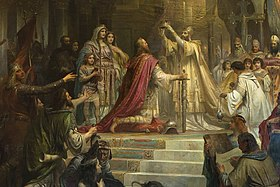
\includegraphics[scale=.5]{a20191225FromClovistoCharlemagne-img001.jpg} 
\end{wrapfigure}

\paragraph{Clovis (466-511)}
Clovis was the first of the 40 kings of France; he united all the Frankish tribes under one ruler. He was Baptized on Christmas Day 496, and three thousand of his companions converted with him.

\paragraph{King Ethelbert}
Pope Gregory the Great, having encountered some young Anglo-Saxons in a Roman slave market, was impressed by their beauty and blonde hair. He sent 40 Benedictine monks, under the leadership of Augustine of Canterbury (as he came to be known) to evangelize the English.

King Ethelbert embraced Christianity. Then he and 10 thousand citizens were baptized on Christmas day, year 597. The king’s baptism was the baptism of an entire people, who gladly followed their leader. From there, St Boniface and several monks set out to evangelize the Germans.

\paragraph{Charlemagne}
A century later, St Boniface was sent from England to evangelize the Germans. Progress was difficult, but after the felled the Donar Oak, without the gods subsequently striking him down, many pagans converted.

Charlemagne became King of the Franks in 768. As the Father of Europe, he re-united most of Roman Europe, even adding new lands to it. Charlemagne was not only a warrior, but the arts and sciences began to flourish again in Europe in the period called the Carolingian Renaissance. He valued learning and education. He encouraged the book publishing on a variety of topics, even founding a library at court. One of his favourite books was Augustine’s \emph{City of God}.

Charlemagne’s Coronation as Emperor of the Romans took place on Christmas day, 800 in Rome. The Roman people acclaimed:

\begin{quotex}
To Charles Augustus, crowned by God as great and pacific Emperor of the Romans, life and victory. 

\end{quotex}

Augustus was the same title claimed by Constantine, emphasizing the continuity between what was to be the Holy Roman Empire with the classical Roman Empire.

\flrightit{Posted on 2019-12-25 by Cologero}

\begin{center}* * *\end{center}

\begin{footnotesize}\begin{sffamily}

\texttt{Cologero on 2020-01-26 at 19:54 said: }

But the recovery of the Mediterranean West is prepared by the Empire of Charlemagne who, through a universal force characteristic of men who hold the spiritual and ethnic-blood heritage of the Romulean lineage, organizes Italy, France and part of Spain: it is strengthened with the supernationalist constitution of the Holy Roman Empire, continues its struggle through the maritime daring of the Maritime Republics of Genoa, Venice, Pisa and Amalfi. \flright{\textsc{Massimo Scaligero}, \textit{La Razza di Roma}}

\hfill
\end{sffamily}\end{footnotesize}

\section{Catching our Breath}

\begin{quotex}
The fool does more harm by his ignorance than the wicked man by his wickedness. \flright{\textsc{Al-Ghazali}}

\end{quotex}

It is time for a recap what has been accomplished thus far in our project to determine the lineament of the Western Tradition, which we claim is as real and as important as anything arising from the East. First of all, we outlined the features of the religion of the Ancient City, how the city was founded by a man-god, its cults, the importance of spiritual authority and its caste based social structure. We showed its decline due to the degeneration of castes which led to the decline of the ancient pagan civilizations due its forgetfulness of its own tradition.

We turned to the next stage of Western tradition, which was both an overthrowing of its decadent predecessor as well as being in continuity\footnote{\url{https://www.gornahoor.net/?p=3281}} with it; this is called Christendom. Ignoring the rather bizarre conspiracies that abound today, we rely instead on \textbf{Rene Guenon}'s sober and intellectually sounder understanding. Christianity at its inception was a mystery religion, founded by a man-god, just as were all the Greek and Roman mysteries and cities. You can accept this claim or not, it has no bearing on what follows. As it became the dominant religion, it was compelled to become exoteric as the social structures of the Roman Empire unraveled. However, we see maintained the outward characteristics of a traditional society: the distinction between spiritual authority and temporal power, as well as a caste based structure with a strong warrior caste\footnote{\url{https://www.gornahoor.net/?p=277}} with its own set of orders. Nevertheless, Guenon insisted on the esoteric character of the dominant spiritual tradition of Christendom, providing many examples from Gospel stories to \textbf{St. Bernard} to \textbf{Dante}, inter alios.

Next, we pointed to Ananda Cooomaraswamy\footnote{\url{https://www.gornahoor.net/?p=556}}, a man whose immense intellect bridged both East and West. He listed several Western authors whose depth of thought rivals that of the East. It would be risable, if it weren't so tragic, to see well meaning men turning to the East while remaining utterly ignorant of the great Western Traditional minds. Please read that piece over and over.

Even \textbf{Julius Evola} had to concede the Traditional nature of Christendom, as much as he disliked its dominant spiritual tradition. Yet, he did make the important point that it was the result of the collaboration of Roman and Nordic elements, the result of which was the spiritual unity of all of Europe, something which did not exist prior to the Middle Ages nor after it following the various reformations and revolutions. His claim that the best aspect of the Middle Ages was its pagan elements is like saying the best part of a cup of coffee is the sugar. They cannot be separated. Furthermore, the spiritual authority defines what it is, which is why Sola Scriptura needs to be rejected.

We then did a creative re-reading of several important figures of Christendom, understanding them as exponents of an esoteric tradition. This, I believe, was very fruitful and it needs to be extended and developed by others. That brings us to the next step which is Guenon's contention that the esoteric tradition has been totally lost in the West, or else it is deeply hidden. We pose the question somewhat differently. First of all, we deny that it has been lost as Tomberg and Mouravieff demonstrate. Whatever their defects may be, they absolutely show the continuing influence of Hermetism, at least in the East of the West. If you doubt the significance of that, please go back to that Coomaraswamy piece and then look up what the ancient Christians wrote regarding Hermes Trismegistus.

The second point is somewhat different. Now, the religion of the Ancient City is certainly lost, in the very real sense that it is unrecoverable — it was lost even at the time of the Roman Empire when men no longer understood their own traditions. The revival is this paganism requires a revelation from a man-god and can never be the result of an artificial reconstruction or re-enactment. On the other hand, the metaphysical teachings of Christendom have not been lost and they even have adherents today. What we can admit, instead, is that the teachings remain virtual, not actual. It would take a gnosis (not a conceptual understanding) to make them actual. However, since they are virtual and not genuinely lost, there remains the possibility of their being actualized. Thus, any objections to self-initiation are beside the point. Anyone confirmed by someone with valid orders has this understanding virtually; under the right circumstances, it can be made effective. We have recently provided examples of the Infinite\footnote{\url{https://www.gornahoor.net/?p=3261}} and the Intellectual Soul\footnote{\url{https://www.gornahoor.net/?p=3390}} which demonstrates beyond a doubt the understanding of the Middle Ages.

Now, we are about to turn to some modern thinkers to show the way from the virtual to the actual. \textbf{Vladimir Solovyov}, who represents the East of the West, was concerned in overcoming the breach between them. As Guenon points out, there is a relationship between theological and metaphysical language. Gornahoor has never engaged in religious polemics, which are pointless. However, Solovyov has developed a metaphysical system which is compatible with his theological understanding. What Guenon hinted at, Solovyov actually accomplished. That is why it is so important to anyone envisioning the religion of the future. Even those who foresee a return to some sort of paganism have to achieve the same level of metaphysical understanding.

\flrightit{Posted on 2011-11-20 by Cologero}

%En The Owl of Minerva, sigue con tres tipos de hombres: Vidente, héroe y creyente. ¿Un capítulo para cada uno en tipos de caminos espirituales?
%Valores familiares, sociales
%Mundo moderno

\chapter{Nobility}
\section{Aristocratic Philosophy}

Several weeks ago I had a conversation with a friend (?) of Gornahoor during which the topic of a ``movement" came up, by which he meant a counter-revolutionary or rightist movement. I had read a post by an alleged leader of said movement that criticized egalitarianism. Following up on that thought, I suggested to my friend that the movement ought to sort itself out by rank. Specifically, if egalitarianism is false, then the different leaders are necessarily unequal. Therefore, it should be possible to determine which are from superior minds and which are inferior. To my surprise, he was appalled by that suggestion. He could only perceive it as some sort of attack, basing his position on the idea that he should be in alliance with those who are ``shooting" in the same direction he is.

But that is begging the question of what is the actual direction of the intellectual bullets. A movement needs to be a microcosm of what it hopes to achieve. Therefore, the movement ought to be clear about its spiritual ideals and its primary exponents, those who would lead, and who are to be the serfs. Otherwise, it is just a mulligan stew, a dish suitable only for intellectual hobos.

Instead of a movement led from above, there is a nebulous mass from below based on little more than popularity, facebook ``likes", and a continuous whir of low quality discussions and arguments. This is the opposite of a hierarchic arrangement. In such an order, a neophyte is not at the same level as an adept. Furthermore, the neophyte is there to learn, not to be ``converted", and certainly not to argue. In order to identify potential members, initiatic organizations have classification schemes to identify various types of men. Certain types cannot qualify for the higher degrees, so it would be pointless to initiate them.

A straightforward classification system is based on worldviews\footnote{\url{https://www.gornahoor.net/?p=3518}}. For example, it is no accident that revolutions arising from the lower classes, as in the French and Russian revolutions\footnote{\url{https://www.gornahoor.net/?p=4235}}, have been explicitly atheist and materialist. Hence, leaders of the ``movement" who are atheist and materialist are vulgar and would most likely belong to a lower caste in a Traditional society.

\paragraph{Philosophic Foundations}
A start in that direction is provided by the short book Nobilitas, by \textbf{Alexander Jacob}, of Indian descent despite his European sounding name. Its subtitle, which describes its aim, is ``a study of European aristocratic philosophy from Ancient Greece to the Early Twentieth Century." It consists of a series of vignettes highlighting the political theories of 20 thinkers, all based on the ideal of the rule by the best. He writes in the Preface:

\begin{quotex}
The superiority of aristocratic government is due not only to its cultural advantage, but also to its solid philosophical foundation. … the term `aristocracy' in my study is not used of a particular class of people so much as of a system of politics devoted to the cultivation of the rule of the best. 

\end{quotex}
By this standard it is eminently fair to demand from the movement an explanation of its philosophical foundation and how the best would be trained and cultivated. Now philosophy, the love of wisdom, is concerned with ideas, hence most of the thinkers mentioned adhere to some form of philosophical idealism. From my point of view, I would have liked to see some medieval thinkers mentioned. Also, since biological racism is not a philosophy, I would replace their representatives in the book with \textbf{Julius Evola} who refuted the myth of blood in favour of the doctrine of spiritual races\footnote{\url{https://www.gornahoor.net/?tag=Sintesi-di-dottrina-della-razza}}. Finally, I would also add \textbf{Rene Guenon}, since his metaphysical teachings would connect Europe to the East.

\paragraph{Gentlemen and Religion}
Now such a short book cannot really describe the philosophical foundations, but only provide some of the more relevant conclusions that arise from them. Not all the thinkers are of the same depth and some are more political thinkers than philosophers in the true sense. However, that is not necessary since the aristocrats would themselves seldom be the philosophers, i.e., the spiritual leaders and educators. Instead, they would be trained in the art of ruling, so the goal of their education is to become gentlemen, not sages. \textbf{Edmund Burke} writes:

\begin{quotex}
Nothing is more certain, than that our manners, our civilization, and all the good things which are connected with manners and with civilization, have, in this European world of ours, depended for ages upon two principles; and were indeed the result of both combined; I mean the spirit of a gentleman and the spirit of religion. 

\end{quotex}
Now, besides the philosophical foundation, we have two new criteria. Which proponents of the movement have the spirits of a gentleman and religion? Are they crude and vulgar, or advocates of a life of sensuality and debauchery? Do they make their case honestly and with integrity or are they full of half-truths and distortions? Is their religious spirit compatible with the history of Europe and the West or do they insist on some mass conversion — or more likely, deconversion — as the precondition for their movement?

\paragraph{Unity of Belief}
Next, is the need for some sort of ``national" unity, however, nation, or nationalism, is defined. Giuseppe Mazzini explains the need for a ``strong national uniformity of thought and faith":

\begin{quotex}
Liberty of belief destroyed all community of faith. Liberty of education produced moral anarchy. Men without a common tie, without unity of religious belief and of aim, and whose sole vocation was enjoyment, everyone sought his own road, not heeding, if in pursuing it, they were trampling upon the heads of their brothers — brothers in name and enemies in fact. 

\end{quotex}
This brings us back to the beginning. Is the ``movement" truly one of real brothers or one of nominal brothers but real enemies? Thus, a movement requires a unity of religious belief. A ``big tent" movement is not organic, but is merely a heap\footnote{\url{https://www.gornahoor.net/?p=1737}}. So what is that belief and how possible is it a force for unity?

So before adopting an intellectual affiliation, investing emotional capital, or even providing financial support, ask if your movement demonstrates these qualities. These are the fruit of a couple of dozen centuries of the aristocratic element in European thought. If you think something ``new" is necessary, or even worse, a new type of man, you will certainly be disappointed. That is why what is required is not a revolution in the opposite direction, but the opposite of a revolution (Joseph de Maistre).


\flrightit{Posted on 2014-01-06 by Cologero }

\begin{center}* * *\end{center}

\begin{footnotesize}\begin{sffamily}



\texttt{William on 2014-01-06 at 10:03 said: }

I've been following Gornahoor for years now, and one example of a fairly pure aristocracy that keeps coming to mind is a proper martial arts dojo. It is easy to settle the question who is better (`aristos’ — let's spar. The sensei is obviously one who knows — he can easily DEMONSTRATE his superior knowledge. The rest of the hierarchy of the dojo is equally easy to settle by the same means. 

Not all dojos are equal, of course — when I started out, I looked for a dojo without a bunch of plastic trophies in the window — competing in local tournaments was not why I was there. And I looked for a sensei with a good heart (a `gentleman’?) — I found one where the sensei had a masters degree in sports physiology and his `day job' was working for the school district developing physical education plans for handicapped kids. Dojos like this are out there.

Looking back on 12 years now, I can say that practicing martial arts has turned out to be a spiritual practice which has deeply changed me for the better. 

In short, the dojo is a living example of a working hierarchy/aristocracy. It has its own Tradition going back millennia. Of course these are small `societies’ — maybe a hundred students at a thriving school? But still, I'm thoughtful what could be learned from them which would apply to the larger questions considered on this site.


\hfill

\texttt{scardanelli on 2014-01-06 at 10:39 said: }

I would say that the major difference is that in physical combat, there is a clear winner and loser whom all can recognize. We can all spar to a greater or lesser degree. When it comes to the esoteric, not all can recognize that which is superior because not all have experience of the esoteric. This knowledge cannot be demonstrated but only experienced within. Therefore those who do not know, do not know that they do not know so to speak.

An aristocracy is based upon the authority of those who have reached certainty within.


\hfill

\texttt{William on 2014-01-06 at 11:30 said: }

I would say that the major difference is that in physical combat, there is a clear winner and loser whom all can recognize

I am not saying that martial arts is a replacement for esoteric work at all. But it is also far more than `physical combat'. All that stuff about `you are your own greatest opponent' is true. There is an enormous amount of `inner' (esoteric) work that a martial artist has to do to progress, including but not limited to overcoming your own ego, overcoming your own fears, being faithful to discipline, humility in the face of a perfection you will never achieve, compassion for students less skilled than you because you need that same compassion from teachers who are your betters, being calm and fully present to your opponent. To me these all sound like spiritual lessons, not physical.

Even in sparring: in a dojo it is not so much about identifying a `winner'. but an opportunity for both participants to try to apply what we've learned. When sparring with a less skilled student, I deliberately emphasize skills I know he is trying to develop. It's a brotherhood.

I'm certainly not suggesting that martial arts is any kind of silver bullet for The Work. But it can be a big help for some, and I still suggest it as a living working example of aristocracy/hierarchy.


\hfill

\texttt{William on 2014-01-06 at 11:38 said: }

For myself, I know I need to submit myself to an authority and discipline greater than myself. So — where to find that? In the context of Gornahoor that would mean the Catholic Church, but where I live the local Catholic Church consists of singing folks songs in spanish to an out-of-tune guitar. And is the priest spiritually developed at all? Having worked as a church musician in churches for 40 years (Protestant and Catholic), I can say that spiritual development correlates poorly to official training and ordination. 

For now, for me, martial arts is the best (though still far from ideal) solution to finding that authority and discipline I know I need.


\hfill

\texttt{JA on 2014-01-06 at 12:04 said: }

``a life of sensuality and debauchery"

How would we explain then Catherine the Great, or the Marquis de Sade, or the Baron von Sacher-Masoch; all of whom were of the best blood ?

I've had the personal honour (or dishonour ?) of being in the same room with members of different royal houses, and honestly brothers – they can snort coke and party all night long as much as any ghetto child……..

Among a certain section of the masses, a careless and libertine way of life is actually associated with aristocracy in their little minds………


\hfill

\texttt{William on 2014-01-06 at 13:49 said: }

I've had the personal honour (or dishonour ?) of being in the same room with members of different royal houses, and honestly brothers – they can snort coke and party all night long as much as any ghetto child……..

Ha ha, precisely! Much the same could be said of cardinals and archbishops (the never ending sex scandals, for openers). Both ecclesiastical AND civil governance is far from `aristos'.

The IDEA of `aristocracy' is great (and all the variations on Plato's philosopher/kings) but how in heaven do we get there?


\hfill

\texttt{scardanelli on 2014-01-06 at 16:02 said: }

William,

I am certainly not denegrating the martial arts. I'm only making the point that the esoteric cannot be demonstrated in the same manner. 

I'm using authority in the sense of Tomberg's fourth letter. Authority is present ``where there is present the breath of sacred magic, filled by the rays of light of gnosis emenated from the profound fire of mysticism." So, where in heaven do we find authority? First learn concentration without effort… This does not necessarily require submitting to the local Catholic Church. At any rate, the whole cannot be judged by the sins of the few. As Cologero has remarked, we get the church that we deserve.


\hfill

\texttt{Michael on 2014-01-06 at 21:06 said: }

I will second what JA says: although I am sure there are exceptions, the aristocrats of the current age show little to no spiritual development.

Will following the path outlined in Meditations on the Tarot lead to a new nobility? Or is spiritual development, at a certain point, incompatible with nobility as we find it in the middle ages?


\hfill

\texttt{Scardanelli on 2014-01-07 at 13:01 said: }

``However, that is not necessary since the aristocrats would themselves seldom be the philosophers, i.e., the spiritual leaders and educators. Instead, they would be trained in the art of ruling, so the goal of their education is to become gentlemen, not sages."

You're right Michael. I should have read more closely.


\hfill

\texttt{JA on 2014-01-07 at 14:32 said: }

amongst many upper class people I know, a pseudo-Nietzschean attitude prevails that personal morality is for the bourgeois, the unenlightened and uneducated folks; and that for those of us of better blood and breeding we are pretty much free to have as much fun and pleasure as we want. In their thinking, the lower classes exist so that we can enjoy ourselves……….and then of course there are those aristocrats who having a ``conscience" and ``compassion" for those less fortunate become leftists.


\hfill

\texttt{Michael on 2014-01-07 at 18:42 said: }

Is the ``pseudo-Nietzschean attitude" the reason we have had the revolution that has resulted in the rule of the shudra? My recollection from Plutarch is that the Roman aristocracy did uphold a higher standard. On the other hand, the ruling class of ancient Greece was immoral in many instances.

The aristocracy of today most likely is just reflecting the degraded morality of the age.


\hfill

\texttt{Matt on 2014-01-07 at 23:25 said: }

``The aristocracy of today most likely is just reflecting the degraded morality of the age."

Or better put, the modern age is just reflecting the degraded morality of the aristocracy. And the term aristocracy is probably not even the right term that applies to the current upper classes, as it means rule of the best; best in virtue and best in intelligence, neither of which the majority of those in the upper class can legitimately claim to represent.


\hfill

\texttt{August on 2014-01-08 at 02:35 said: }

It doesn't matter what one does. Who cares about morality, especially now. The important part is what motivates him to do it, what is happening inside. If you have to persistently restrain yourself from a loose lifestyle, how are you any better from someone who indulges similar impulses? At most you've demonstrated better self-control, in the worst case it's just a matter of time until you relapse or some monstrous repression erupts in one fashion or another. And at least you know what you're dealing with in the presence of the openly indulgent.

When you have crossed a threshold, you know it because even if you WANT to, say, party like you did when you were a 20 year old, there is no longer anything inside you to allow you to do it. Sure, go buy some drugs and head to the club, but you may as well be baking muffins for all the inner participation that is taking place, and going through stupid motions quickly makes one feel stupid. When the inner mania evaporates, the superficial desire quickly goes too, and no restraint is required. Do you see why some people fear a spiritual correction more than death?

If `aristocrats' aren't getting to this point, it could have something to do with the active tendencies, and vanity, of their class, which in our bland surroundings find convenient expression in the artificial drama-world of the drug-sex-party social complex. That they can't see how pathetic it is to get bogged down in that and actually enjoy it is also perhaps to be expected, given that they historically relied on spiritual authority for direction. It also seems to be, originally, a signature British weakness.


\hfill

\texttt{Scardanelli on 2014-01-08 at 15:36 said: }

In what sense are you using morality august? Perhaps I'm misunderstanding you. Morality isn't just an arbitrary law imposed upon ones ego from without and masking ones true depravity, but an expression of an inner state reflected in the outer. Thus morality is relevant in that when we act in a moral way, our wills are aligned with providence and impose this upon destiny, so to speak. Therefor it does matter what one does… To be moral is to redeem the flesh, to spiritualize matter.


\hfill

\texttt{August on 2014-01-08 at 18:09 said: }

Though it should have been obvious from the lines following, I was referring to morality in the Protestant sense, an arbitrary behavioural convention, a residue, given excessive importance and divorced from real ties to the spiritual, eventually failing in its only potentially useful role of maintaining a kind of public order.


\hfill

\texttt{Cologero on 2014-01-08 at 21:11 said: }

On the word of a modern day Greek aristocrat (Joy is a state of mind), drinking, debauchery, and sports competition are sources of joy if done with good breeding, style, and manners. A gentleman understands moderation, so he doesn't go to the extremes of a saint, yogi, or even philosopher.


\hfill

\texttt{Michael on 2014-01-09 at 18:17 said: }

Cologero, Taki is a charming guy, and I think he is in many ways a good model, but how does debauchery fit in with theosis? Isn't the goal still to ``be perfect as your heavenly Father is perfect?"


\hfill

\texttt{Gina on 2014-01-17 at 11:49 said: }

Engaging post. This statement about the favoring of spiritual races over biological ones rings true in my opinion. I've felt it creates a problem in the modern day. Good breeding, higher education, and a deeper appreciation of sciences and art are all something that leaders should possess, and these are qualities that are not blood inherited, although money helps when on the road to spiritual attainment (in my opinion). 

Many people can legitimately trace their family lines back to royalty. I am one of them. This doesn't make them great leaders or worthy to live off of tax payer money. I'd say this is a gross misuse of funds. 

In Kabbalah, for instance ``House of Jacob" is somewhat equal to saying ``soul of balance". The middle way. An aspect coming from Tiphereth. I also do believe that Jacob was historical, however, if you can trace your lineage back to him, you're just as likely to be a King in Saudi Arabia as you are to be an accountant. Certain ``Houses" meant spiritual grades in old times. We've become quite Pharisaic maybe in our interpretation of these hierarchical systems.

Good genes or potentially good epigenetic conditions are not hoarded in royal houses or amongst those in the elite bourgeois. However, our society seems to have destroyed the tenets by which purposeful mating was made important. I do see that. This is a bit of a religious and social crisis where the spirituality has been sucked from the materiality.


\hfill


\hfill


\hfill


\end{sffamily}\end{footnotesize}

\section{Prole Thoughts}

Since I had been taking notes about various news programs over the past week, I was intending to comment on them. That turned out to be distasteful and probably futile, so instead I prefer to continue commenting on European aristocratic philosophy as succinctly summarized by Prof \textbf{Alexander Jacob} in his book \emph{Nobilitas}; since it seems to be unavailable, there is all the more need to do so.

Many contemporary historians have lamented the lack of direct documentation provided by the ``common" people of past generations. Hence, they go looking for letters to soldiers, or diary entries, etc., to fill in that gap. Today, there is no such problem at all. On the contrary, ``prole thoughts" are all too available through the so-called ``social media" of facebook, twitter, huffington post, and so on. Their interests, concerns, activities, and forms of thought are available for the next great historian of our age to digest. This, however, must be much more than a mere statistical study.

A half step up are found the poseurs. Not content with common interests, they use social media as a debating platform for politics, philosophy, religion and related erudite topics. Since it is impossible today to master all human knowledge, the days of the Renaissance Man are long gone. Nevertheless, most people feel competent to make definitive judgments on complex issues of science, economics, ethics, sociology, and psychology. You would think a lifetime of average grades and standardized test results would discourage people, but it seems not to be the case. Without a teacher, everyone imagines himself capable of ``A" work.

That is likely because at adulthood, his worldview is firmly set, for better or worse, and any challenge to it results in psychic distress. That is why such social media discussions often turn nasty. Someone once said that most men hold opinions that can each fit onto a placard. So a half dozen or so disconnected placards contain the framework for their entire life of the mind. The details don't matter, since any content can be reframed within that framework, like some Procrustean bed. \emph{Nobilitas} is intended to reach the one in two hundred men who are not satisfied with placards.

\paragraph{Rule of the Best}
Based on some recent comments, let us be clear what this means. The best are well born and well educated. Well born does not mean having the best parents, so strictly speaking it is not always a matter of a bloodline. Furthermore, to be ``educated" means to have wisdom developed from within. In short, the raw matter must first be there and then it must be developed; obviously, a healthy social structure will develop such talent. This is contrary to the tabula rasa ideal of today in which everyone is considered to be born equal, and the task of education is to implant the right ideas into that empty space. I should mention at this point that the Greek ideal can also be found in the East, for example, in \textbf{Shankara}'s \emph{Crest Jewel of Discrimination}.

Starting with the Greeks, we see the themes of the One, the Good, and the Logos. The wise man is one who can see the unity of spirit in the multiplicity of manifested things. The highest idea is the idea of the Good and the Logos or cosmic order is an object of contemplation. As we saw last time via Giovanni Gentile, the intellectualism of the Greeks gives way to the voluntarism of the Christian era. In the latter, there is the same understanding of the One; however, the Good becomes Love and the Logos is no longer object but becomes subject. Moreover, Jung claimed that ``individuation" was possible only in certain cultures. Keep these thoughts in mind in the historical manifestations of aristocratic philosophy.

Since modern ideals are so ingrained in nearly everyone today, it may be difficult to understand or come to terms with aristocratic philosophy. For example, the first principle is that the superior rules the inferior; in particular, the lower desires are to be ruled by the dictates of reason. On the contrary, today's standard is that the purpose of reason is to lead to the satisfaction of lower desires. In particular, the conventionally intelligent\footnote{\url{https://www.gornahoor.net/?p=1582}} mark themselves by being sexually risqué, as though they can't find any other purpose for their intelligence.

In the social realm, the same principle holds. Plato claimed that untrained passions are found in children, women, and lower classes. Apart from children, perhaps, such a claim is now rejected, even as passion itself is celebrated. In particular, any movements that claim to be recovering the aristocratic philosophy ought not be run and organized by women.

I have noticed the tendency of some self-described elitist movements that have disdain for lower classes. On the contrary, the Greek model was the common good; society was to be organized even for the benefit of the lower classes. Actually, the philosophical elite, which corresponds to the traditional idea of the Brahman class, has little need for what pleasures the rest of society. Hence, the ruling elite have no need for sexual or financial exploitation, unlike what is found in all modern social systems. \textbf{Plato}'s \emph{Republic} would be ruled by a philosopher-king. Prof Jacob quotes Plato:

\begin{quotex}
Unless either the philosopher become kings in our states or those whom we now call our kings and rules take to the pursuit of philosophy seriously and adequately, and there is a conjunction of these two things, political power and philosophic intelligence, while the motley hordes of the natures who at present pursue either apart from the other are compulsorily excluded, there can be no cessation of troubles for our states nor for the human race. 

\end{quotex}
This is somewhat different from \textbf{Rene Guenon}'s view of the separation of spiritual authority from political power. The philosophers are the spiritual leaders, advisors, and educators, but few have the talent, or even the interest, for ruling. Hence, kings must be educated in the proper philosophy and willing to follow the direction of the philosophers. This system as such was not fully tried in the West until the Middle Ages in which the role of the philosopher was that of the Church and the king's legitimacy depended on the spiritual authority.

As for Plato's prediction of troubles for the human race if his ideal was not followed, can there be any doubt? Since, in the West, many have found pockets of stability, they are unaware of such problems and have scant sympathy for the actual victims of such troubles.

Of existing forms, Plato insists that kingship is the best provided there is rule of law. This is contrary to \textbf{Julius Evola}'s opinion\footnote{\url{https://www.gornahoor.net/?p=6548}} that leaves no space for a separate spiritual authority in the monarchy and allows the monarch absolute power. However, for Plato and the Medievals, the positive law must be consistent with the cosmic law.

\paragraph{Rule of the Gentleman}
The other Greek thinker treated by Prof Jacob is \textbf{Aristotle}, who has a slightly different conception. While Plato's system goes to extremes, Aristotle recommends moderation. For Aristotle, the national good is superior to the merely individual good. Such a position is difficult to defend today in the West since the idea of a nation is mostly discredited. Hence, Western political systems are organized around providing goods and services to particular individuals based only on their political influence. However, this is only partly true, since various subnations, based on race, ethnicity, religion, or even behavioral preferences, vie for goods apart from the good of the body politic as a whole.

Although Aristotle believes everyone should strive for the mean, there are still those who are superior and those who are inferior. A gentleman would be magnanimous, virtuous, just, and prudent in knowing how to apply higher principles to political life. He develops friendships among men of similar character.

Now, this is a sound corrective to Plato. A ruler ought not be as extreme or fanatical as Plato's guardians. This was the position in the Middle Ages, in which the nobility held the place of the gentleman. While a St. Francis of Assisi may be a model for the spiritual class, it is not intended as the proper way to rule a society. Unfortunately, fanaticisms of various types have been commonplace in the turmoil of the modern world.


\hfill

Next: Rome and the Renaissance



\flrightit{Posted on 2014-01-12 by Cologero }

\begin{center}* * *\end{center}

\begin{footnotesize}\begin{sffamily}



\texttt{JA on 2014-01-13 at 09:53 said: }

This series is very informative and much needed, I look forward to the subsequent chapters.


\hfill

\texttt{Avery Morrow on 2014-01-13 at 11:39 said: }

``While a St. Francis of Assisi may be a model for the spiritual class, it is not intended as the proper way to rule a society."

Honestly — even if someone happened upon this proper way to rule, who of this era would want to listen to them? Perhaps all we have left at this point, lacking any acceptable guidance from the old social elites, are pointers back to the unrefined Tao.


\hfill

\texttt{Michael on 2014-01-16 at 22:01 said: }

I think the book is an excellent introduction to the topic, but it leaves me wanting to learn more. Does anyone have any suggestions for reading how aristocracies are established in the first place?


\hfill

\texttt{Cologero on 2014-01-16 at 22:57 said: }

Yes, Michael, that is the point and it will be covered shortly. By way of introduction, I can make the following points.

First of all, it must be stipulated that the civilization of the Middle Ages represents in the West the closest approximation to a Traditional civilization as described by Guenon. Anyone who will give the matter at least serious consideration can hardly deny it.

So we can focus on its beginning stages so we can learn from it. The knights represent the ideal of the gentleman and the monks were closest to the philosophers, i.e., those dedicated to a higher calling above material and sensual pleasures. Plato's further division of the Republic into warriors and producers mirrored the Middle Ages.

The creators of the civilization of the Middle Ages were the \emph{true} men among the ruins, i.e., of the Roman Empire. For them, it was a matter of life or death, not an effete intellectual theory as it has become today.

The social hierarchy was both consciously and unconsciously created and arose organically for the most part. Strong leaders such as Clovis and Charlemagne, established and protected that hierarchy. Certain intellectual currents, originating from the poets and religious authorities, provided the justification. We addressed that topic specifically over a year ago in \textit{Pray, Fight, Work}\footnote{\url{http://www.gornahoor.net/?p=5198}}, even if no one then seemed to grasp its significance.

Now there are many other explanations for this, but they do not take into account the true nature of a Traditional civilization and social organization.

As for the ``how" … a Traditional civilization depends absolutely on an authentic Tradition. That is the ineluctable foundation which the Middle Age civilization was blessed with, and that foundation cannot be based on vague imaginings or unsupportable speculations. Without that, there is nowhere to go.


\end{sffamily}\end{footnotesize}

\section{Prolegomena to Noble Philosophy}

\begin{quotex}
Nobility, the quality which I call true aristocracy, requires of a man the recognition of his guilt. In its depths, conscience, which is frequently covered up and suppressed, is always a consciousness of guilt. The necessary thing is to take upon oneself as much guilt as possible and to put as little as possible of it upon other people. The aristocrat is not one who is proudly conscious of himself as first, as a privileged being, and who safeguards his position as such. The aristocrat is the man who is aware of the guilt and sinfulness of this first place, this privileged position of his. \textit{The sense that one is being continually affronted is on the other hand, precisely a plebeian feeling}. \flright{\textsc{Nicolai Berdyaev}}

\end{quotex}
I've been away with severe bronchitis, probably resulting from a pneumothorax I suffered two months ago. I tried the auto-suggestion exercise, but was unable to achieve any lasting results. I found it difficult to reach any transcendent state as gasps for air brought me back. Of course, on the physical plane, possibilities may be exhausted in a process of densification. Despite trying ayurvedic and Santeria home cures, (everyone had an opinion), I eventually turned to heavy doses of white man's medicine. Interestingly, while the body is still subpar, there was a specific spiritual healing which I shall keep to myself.

In that time, I considered several ways to return to the topic. Specifically, what can we glean from the documentation we have on the formation of Tradition in the middle ages? This will require a review of the historiographical method as well as a refresher on the \textbf{Ancient City}. Although I like \textbf{Alexander Jacob}'s term ``aristocratic philosophy", the title of his book, Nobilitas, better suits the purpose. The original term may be misleading, since it is a philosophy for aristocrats, not from aristocrats. After all, an aristocrat is a gentleman and therefore ill-suited to the nitpicking of critical philosophy. So while a \textbf{Socrates} is debating the meaning of courage, piety, justice, etc., in thought, only to end up in aporia, the aristocrat is effecting those virtues in being. He strives to ``be" courageous, pious, just, and so on. Although I would prefer to use the Sanskrit word for noble\footnote{\url{http://www.behindthename.com/name/arya}}, the English ``Noble Philosophy" will suffice for obvious reasons.

Yet even the word ``philosophy" is misleading, since profane philosophy has come to mean something critical or speculative rather than a way of life. That is why Guenon distinguished between metaphysics and philosophy, yet ``Hermetic philosophy" is actually metaphysics. Profane philosophy represents a decline, since it attempts to do in thought what had been accomplished in being.

In Professor Jacob's study of aristocratic philosophy, there is a gap between ancient philosophy as represented by \textbf{Plato}, \textbf{Aristotle}, and \textbf{Cicero}, and the Renaissance and later thinkers. In a sense, profane philosophy represents decadence and a decline from more traditional thought. Thus, Plato created a republic in thought, whereas the ancient Greek city created them in reality. Those cities were established by a godling or man with divine qualities. They were initially ruled by a priest-king and religious rites organized the life the city and its inhabitants. Aristotle presumably had access to those ancient constitutions from which he developed his political philosophy. Cicero admitted he could not understand the ancient Roman customs and laws.

\textbf{Ulrich Valange} observed that High Culture requires culture creators and culture sustainers. So in the Ancient City, the founders were the creators and the nobility were the sustainers, so long as they kept the hearth burning. The clients, or plebes, had no culture of their own and simply followed the culture and rites of their particular ruling family. In this sense, therefore, the culture was ``imposed" on them. This relates back to Berdyaev's opening quote.

The esoteric method is neither argumentative nor empirical. Rather, it is descriptive, since to know requires an intuition, that is, something more like seeing. It is based on principle, so we don't reason from the many to the One, but instead we strive to understand the many from the One. Hence, the principle of the Ancient City, as it relates to High Culture, manifests as creators, sustainers, as well as the passive elements. We are not interested in the faux debates among these groups, but rather in observing how they manifest the principle.

The true aristocrats are acutely aware of their role as the culture sustainers and strive to fulfill that role. Whenever there is a failure in some regard, they become ritually unclean and need to restore the balance. Initially, this was exteriorized, but becomes interiorized in the Middle Ages as we shall see. They are motivated by honour and duty, not by their ability to dominate, although they exercise the power of command as necessary.

Lower than them, are the plebes. They can neither fully understand nor participate in the culture. Hence, they become prone to feelings of ressentiment. They feel that something has been ``imposed" on them. We see that especially in certain neo-pagan circles, who complain that medieval Christianity was forced on them. Understand, from our perspective, that it is pointless to engage in some mock interminable debate; rather, we simply see what type of person holds what type of worldview. As a reminder, from the esoteric point of view, this is what \textbf{Rene Guenon} wrote, (regarding whether Dante was a Catholic or a pagan):

\begin{quotex}
For our part, we do not think that such a point of view is necessary, for true esoterism is something completely different from outward religion, and if it has some relationship with it, this can only be insofar as it finds a symbolic mode of expression in religious forms. Moreover, it matters little whether these forms be of this or that religion, since what is involved is the essential doctrinal unity concealed beneath their apparent diversity. 

\end{quotex}
Those who feel victimized, then, simply do not and cannot understand this. The prime example, as we have repeatedly pointed out, is the legend of the Virgin Spring\footnote{\url{https://www.gornahoor.net/?p=1416}}; there we see the aristocratic and plebeian characteristics fully revealed. These are not judgments; rather they are descriptions of certain states of consciousness.

Next: The Foundation of the Middle Ages.

\flrightit{Posted on 2014-02-13 by Cologero }


\chapter{Return to Tradition}
\section{Lightning Strikes from the East}

\begin{quotex}
Ignorance pure and simple is far preferable to false ideas. \flright{\textsc{Rene Guenon}}

Lightning cometh out of the east, and appeareth even into the west. \flright{\textsc{Jesus Christ}}

\end{quotex}
In \textit{East and West}, \textbf{Rene Guenon} outlines a plan for the recovery of Tradition in the West. Obviously, the plan is complex and requires some unique skills as well as intellectual depth to succeed, and it is something he doesn't expect to happen next week. Nevertheless, it is well worth elucidating in detail, if only for the boons it will bring to those who make the effort to understand. However, we take it seriously as we heed Guenon's warning\footnote{\url{https://www.gornahoor.net/?p=35}} about the consequences of not undergoing a consciously led social transformation. These are either a fall into complete barbarism or else the assimilation to another Traditional culture, most likely following a period of social upheaval. The plan must take place on three levels:

\begin{enumerate}
\item The knowledge and understanding of metaphysical principles 
\item The recovery of traditional sciences 
\item The transformation of the social order 
\end{enumerate}
\paragraph{Return to Intellectuality}
First of all, it is necessary to understand the goal, or what exactly defines a traditional civilization. Guenon explains:

\begin{quotex}
What we call a traditional civilization is one that is based on principles in the true sense of the word, that is, one where the intellectual realm dominates all the others, and where all things, science and social institutions alike, proceed from it directly or indirectly, being no more than contingent, secondary and subordinate applications of the purely intellectual truths.

\end{quotex}
To be blunt, the intellectual truths he is talking about are not debating points; they are either understood or they are not. The thinking, willing, and feeling functions must be understood in their proper relation. This is especially true in our age with its emphasis on action for its own sake and sentimentality. Guenon writes:

\begin{quotex}
The pure idea has no immediate relation with the domain of action, and it cannot have the direct influence on outward things that sentiment has; but the idea is, none the less, the principle, the necessary starting point of all things, without which they would be robbed of any sound basis. Sentiment, if it is not guided and controlled by the idea, brings forth nothing but error, disorder, and obscurity; there is no question of doing away with sentiment, but of keeping it within its legitimate bounds.

\end{quotex}
The dominance of sentimentality is expected in the modern mind, but it seems to be none the less present even among some segments seeking a return to tradition. So we must insist on this initial understanding, as Guenon explains:

\begin{quotex}
Thus a return to tradition and a return to principles are in reality just one and the same thing; but clearly the knowledge of the principles, where it is lost, must first be restored before there can be even a remote thought of applying them; it is quite out of the question to build up again a traditional civilization in all its fullness without first having the supreme and fundamental knowledge that must preside over the work.

\end{quotex}
\paragraph{Return to Tradition}
Since the time Guenon's book was published, much has changed in the West. On the one hand, the knowledge of Eastern systems such as the various schools and sects of Hinduism as well as Buddhism, has become much more prevalent, even to the point of attracting many adherents. On the other, there are the many alternative, or New Age, types of spiritualities, primarily deriving from Theosophy and similar movements. The latter consist of a strange mix of not fully understood principles heavily infused with mushy sentimentality. The former, although they show some promise, are too often incompatible with the Western mindset and style of life. The adherents either adopt alien styles of dress and mannerisms which are quite secondary to the intellectual principles or else end up accommodating the Eastern teachings to Western prejudices and, in the process, compromising what is authentic in them. That is why Guenon suggests:

\begin{quotex}
In our eyes, the most satisfactory solution for the West is the return to her own tradition, completed where necessary as to the domain of pure intellectuality.

\end{quotex}
Now, this requires some explanation since the Western mind is so imbued with egalitarianism, even among those most loudly calling for a return to Tradition. This domain of intellectuality is only suitable for the small minority, or elect, who are capable of understanding. For the rest, there needs to be an exoteric religion that bears these principles in a more palatable form. Hence, we witness the many discussions, often heated, about a return to Christianity or some sort of neopagan revival. That debate is not of interest to the elect who understand that metaphysics and religion need not be in the least incompatible. Guenon writes:

\begin{quotex}
Even if the West repudiates sentimentalism (and we mean by that the predominance of feeling over intelligence), the western masses will retain none the less a need for satisfactions derived from sentiment, which the religious form alone can give them, just as they will retain a need for outward activity.

\end{quotex}
There are certainly some manifestations of Western thought that are of a high intellectual caliber. Unfortunately, they are ignored by contemporary leaders of the Western religion who falsely believe they are in continuity with that tradition. Or else, they are depreciated and rejected by others because the Western tradition is ``\emph{too high for them}", as Guenon writes. The latter go searching in vain for an elusive ``authentic" tradition, when they can't even understand the one that is closest in time to them. We will bring what Guenon has to say on this topic at a later date.

\flrightit{Posted on 2012-01-17 by Cologero }


\chapter{The Western Tradition}
\section{The Esoteric Path}

\begin{quotex}
In this case it would be better, although not absolutely necessary, for the elite to be able to take as its basis a Western organization already enjoying an effective existence. It seems quite clear that there is now but one organization in the West that is of a traditional character and that has preserved a doctrine that could serve as an appropriate basis for the work in question, and this organization is the Catholic Church. It would be enough to restore to the doctrine of the Church, without changing anything of the religious form that it bears outwardly, the deeper meaning that is truly contained in it, but of which its present representatives seem to be unaware, just as they are unaware of its essential unity with the other traditional forms. \flright{\textsc{Rene Guenon}, \emph{The Crisis of the Modern World}}

\end{quotex}
\paragraph{Western Tradition}
It was Guenon's position that, at least for those at a sufficient level of development, the choice of an esoteric path was a matter of personal choice and opportunity. In \textbf{Boccacio}'s \emph{Decameron}, which Guenon regarded as the work of an initiate in the same Tradition as Dante, there is the story of the three rings. In that tale the true religion, between Judaism, Christianity, and Islam, was represented by a golden ring. In the tale, two identical copies were made making it impossible to tell which of the three was the true religion. There are three possible interpretations of the story.

Nevertheless, Guenon thought that the Catholic Church was the natural basis for the re-establishment of Tradition in the West. Obviously, not as it was constituted, but presuming that a spiritual elite might arise who could restore the deeper meaning contained therein. In several of his early works, he provided clues to what they may look like.

We have mentioned Guenon's writings on the Crown of Creation \footnote{\url{https://www.gornahoor.net/?p=7768}} as the basis for metaphysics and the Social Reign of Christ as the model for social organization. This is not the place for details, but it is certainly sufficient as a sound beginning for the restoration.

Certainly, it is a sound project to investigate the Medieval period as a model since all writers of Tradition regard that age as the most recent Traditional civilization in the West. Although Guenon saw its demise in the Renaissance, Evola referred to what ``every well born man considered sane and normal prior to 1789." The spiritual basis of that sane and normal time is irrefutable.

Guenon believed that the revival of Thomism following Pope Leo XIII's encyclical left out an important element. Specifically, Thomism became too dependent on Aristotle, while leaving out the more important influence of Neoplatonism, Augustine, and Dionysus. In this he was opposed by Jacques Maritain who even lobbied to get Guenon's books place on the Index while he was the French ambassador to the Vatican. Therein lies a clue to the possible restoration, which should be further enhanced with a dialog of more the more ancient Vedic teachings.

\paragraph{Adoption}
The three Western traditions are in continuity. We have pointed this out several times: Christianity is esoteric paganism\footnote{\url{https://www.gornahoor.net/?p=7152}}, Augustine referred to the one Tradition, Dante built on Virgil. More recently, \textbf{C S Lewis}, \textbf{Valentin Tomberg}, and \textbf{Joseph Ratzinger} regarded Christianity as the fulfillment, not only of the Hebrew religion, but also of paganism.

The idea of a new people founded by a God-man was not unknown at that time and would have colored the understanding of early Christians. In his studies of the spirituality of Ancient Rome, Evola focused exclusively on a given bloodline. However, birthright was not the only means to participate in a spiritual stream. A man who had no male heir was able to adopt one into his family. From the spiritual point of view, that served the same purpose.

For example, Romulus was the demigod son of Mars; this is not totally fictional since the martial spirit of Rome certainly existed, however you want to understand that. However, Jesus Christ was the Son of a virgin and of the Holy Spirit, hence, not a particular god of a certain spirit, but the Absolute God of all creation. This started a spiritual race, not of blood, but from adoption. We become sons of God by adoption. Sons share in the nature of their fathers and are entitled to an inheritance. This is much more than mere creaturehood. In our time, this notion has been sentimentalized to turn believers into perpetual children.

\paragraph{Initiation}
Guenon insisted that a valid initiation was necessary for an initiatic path; the validity was guaranteed by an unbroken chain of initiates. Certainly, this is not sufficient since Guenon himself pointed to several Hindus and Sufis who proclaimed heterodox doctrines despite their initiations.

Evola criticized Guenon in that regard for the bureaucratization of initiation. More important than the horizontal was the vertical, so Evola proposed that there was an initiation from above. He never really identified that. Tomberg, however, wrote that all initiation is from above and is the second birth in Christ.

Thus, in the West, Hermetic groups appear and go dormant, without a visible continuity. That is so it does not become as sort of counter-Church.

\paragraph{Buddhism}
\begin{quotex}
Guenon has made a commendable effort to interpret the true spirit of Hindu culture to the West in his many works … The form of regeneration consists not in a fusion or synthesis of the two cultures, but in the West regaining, as the result of a dynamic turn in its present trend, those springs of true spirituality through the help of the East. It would be hazardous to forecast the time of the change or the precise manner in which it would be brought about. \flright{\textsc{T R V Murti}, \emph{The Central Philosophy of Buddhism}}

\end{quotex}
However, about 20 years ago, I took Guenon's point very seriously. If it was true that there was no available initiation in the West, I searched for another, which came done to taste and opportunity. I had a romanticized vision of Tibet. There were the tales from Alexandra David-Neel, the Roerich's, not to mention the various claims of the occultists. Tibet had been the last patriarchal, hierarchical, theocratic society. Since there were a few Tibetan centers locally of different lineages, I decided to get initiated at one of them, in the tradition of the \textbf{Dalai Lama}.

So for a few years, I followed that path. It was not so different. There was a priest, an altar, flowers, incense, a rite, veneration of relics, icons, prayers, meditations, heaven, hell, and a period of post-mortem purgation. I followed the precepts of the vows, which were very much like the Tao described by C S Lewis. A minor transgression, or ``venial sin", could be rectified by suitable prayers. A ``mortal sin", such as stealing a freight train or having anal intercourse with your wife, put you outside the sangha and could only be rectified by retaking the vows.

Nevertheless, virtually every Westerner I met told me how they had surpassed the religion of their upbringing. From a practical point of view, I couldn't see much difference. Clearly, they were ignoring several points of the vow. Instead, becoming a vegetarian or rescuing a dog from the pound became the main focus.

I never heard anyone of them advocate the desirability of a patriarchal theocratic Buddhist state in the West. Even the Dalai Lama ended the reincarnations of future Dalai Lamas and came to prefer a Euro-style parliamentary system for any future free Tibet. Hence, it was time to leave.

Can it be said that the initiation really made any difference, beyond a post hoc, propter hoc argument? Certainly the many hours spent in meditation with mala beads and the study of Madhyamika must have accomplished something. At the very least, it was the ``help from the East" that Guenon claimed was necessary.

I am not recommending this choice, since I see that the same, or more, can be accomplished within the Western Tradition. Buddhism is a paganism and thus can be superseded while absorbing its best practices and metaphysical teachings. Then there is the matter of recognizing the real ring.



\flrightit{Posted on 2015-02-09 by Cologero }

\begin{center}* * *\end{center}

\begin{footnotesize}\begin{sffamily}



\texttt{Cologero on 2015-02-12 at 20:54 said: }

I appreciate your comments, Mr Obscure, but I need to keep making the same point over and over again. The Tradition is one thing, the current management is another. That is a distinction to always keep in mind, especially given Guenon's claim that the current leaders are not likely to be aware of the full Tradition. As I've tried to show , this is not an idle opinion … Guenon did indeed try to reinvigorate Tradition. There is also the model of Guido De Giorgio with his ``Vedantized Christianity" as Evola called it.

I agree with your points, but what I reject is that we have to wait for George to do it\footnote{\url{http://en.wikipedia.org/wiki/Let_George_Do_It_\%28radio\%29}}. We do not need more kibitzers and complainers, but men of action. This is George's motto:

\begin{quotex}\footnotesize
Personal notice: Danger's my stock in trade. If the job's too tough for you to handle, you've got a job for me. George Valentine. 

\end{quotex}
Is that clear enough?


\hfill

\texttt{Cologero on 2015-02-12 at 21:03 said: }

I'll iterate these points since new readers may not have encountered them yet.

Evola developed an interest in Idealism (it was the dominant Italian philosophy at the time), so he taught himself German so he could read all the German Idealists (and Nietzsche). From that, he created his own philosophical system while still a young man. He was not concerned about any ``suspicion" that his system would arouse.

A second point. Do you think that God chose Joan of Arc, a young woman, to save France? Not at all. First He went down the list but all the men, one after the other, refused the task. As He neared the bottom of his prospects, she was the only one not to refuse. I bet there is a lesson there.


\end{sffamily}\end{footnotesize}


\end{document}
